\chapter{Mapping human health risks from exposure to trace metal contamination of drinking water sources in Pakistan}
\label{chapter5}

Avit Kumar Bhowmik\textsuperscript{a}, Ambreen Alamdar\textsuperscript{b}, Ioannis Katsoyiannis\textsuperscript{c}, Heqing Shen\textsuperscript{b}, Nadeem Ali\textsuperscript{d}, Syeda Maria Ali\textsuperscript{e}, Habib Bokhari\textsuperscript{f}, Ralf B. Schäfer\textsuperscript{a}, Syed Ali Musstjab Akber Shah Eqani\textsuperscript{f}\\[.5cm]

\small

\textsuperscript{a}Institute for Environmental Sciences, University of Koblenz-Landau, Fortstrasse 7, D-76829 Landau in der Pfalz, Germany.

\textsuperscript{b}Key Lab of Urban Environment and Health, Institute of Urban Environment, Chinese Academy of Sciences, Xiamen 361021, PR China.

\textsuperscript{c}Aristotle University of Thessaloniki, Department of Chemistry, Division of Chemical Technology, Box 116, Thessaloniki, 54124, Greece.

\textsuperscript{d}Department of Environmental Sciences, FBAS, International Islamic University, Islamabad, Pakistan.

\textsuperscript{e}Center of Excellence in Environmental Studies, King Abdulaziz University, Jeddah, Saudi Arabia.

\textsuperscript{f}Public Health and Environment Division, Department of Biosciences, COMSATS Institute of Information Technology, Islamabad, Pakistan.\\[1cm]

\medskip

\normalsize
\noindent Adapted from the article published in 2015 in Science of the Total Environment\footnote{Science of the Total Environment is the one of the most important scientific journals in the field of environmental science that publishes original research on total environment. The current impact factor of the journal is 4.099 according to the Journal Citation Reports, 2015 (\href{http://wokinfo.com/products_tools/analytical/jcr/#}{http://wokinfo.com/products\textunderscore tools/analytical/jcr/#})}, vol. 538, pp 306-316.\\[.5cm]

\renewcommand{\abstractname}{Abstract}
\begin{abstract}
The consumption of contaminated drinking water is one of the major causes of mortality and many severe diseases in developing countries. The principal drinking water sources in Pakistan, i.e. ground and surface water, are subject to geogenic and anthropogenic trace metal contamination. However, water quality monitoring activities have been limited to a few administrative areas and a nationwide human health risk assessment from trace metal exposure is lacking. Using geographically weighted regression (GWR) and eight relevant spatial predictors, we calculated nationwide human health risk maps by predicting the concentration of 10 trace metals in the drinking water sources of Pakistan and comparing them to guideline values. GWR incorporated local variations of trace metal concentrations into prediction models and hence mitigated effects of large distances between sampled districts due to data scarcity. Predicted concentrations mostly exhibited high accuracy and low uncertainty, and were in good agreement with observed concentrations. Concentrations for Central Pakistan were predicted with higher accuracy than for the North and South. A maximum 150-200 fold exceedance of guideline values was observed for predicted cadmium concentrations in ground water and arsenic concentrations in surface water. In more than 53\% (4 and 100\% for the lower and upper boundaries of 95\% confidence interval (CI)) of the total area of Pakistan, the drinking water was predicted to be at risk of contamination from arsenic, chromium, iron, nickel and lead. The area with elevated risks is inhabited by more than 74 million (8 and 172 million for the lower and upper boundaries of 95\% CI) people. Although these predictions require further validation by field monitoring, the results can inform disease mitigation and water resources management regarding potential hot spots. 
\end{abstract}

\newpage
\thispagestyle{empty}

\vspace*{\fill}
\begin{quotation}
  \large\textit{``Sooner or later, we will have to recognise that the Earth has rights, too, to live without pollution. What mankind must know is that human beings cannot live without Mother Earth, but the planet can live without humans''}.
   ---Evo Morales
\end{quotation}
\vspace*{\fill}

\newpage

\section{Introduction}
\label{Introduction}

Inland ground and surface water are globally important drinking water sources, which are influenced by natural and anthropogenic processes. These can result in elevated levels of different contaminants in drinking water (Winkel et al., 2008; Shah et al., 2012). Several pathogens as well as organic and inorganic components occur in drinking water sources of many regions of the world and may have acute and chronic effects on consumers' health (Srinivasa and Govil, 2007; USEPA, 2014). For example, one-third of annual mortality in Pakistan has been attributed to drinking water contaminated by microbial and/or chemical components (Azizullah et al., 2011).

Trace metals represent a major group of contaminants of drinking water sources that can have severe implications for human health, e.g., cardiovascular and skeletal diseases, infertility and neurotoxicity (WHO, 2011). In developing countries, contamination of drinking water sources by trace metals have been triggered by rapid industrialization and excessive usage of pesticides and chemical fertilizers in agriculture during the last decades (Srinivasa and Govil, 2007; Farooqi et al., 2008;  Eqani et al., 2012). In addition, geogenic sources contribute to the wide occurrence of trace metals such as arsenic in ground and surface water (Winkel et al., 2008). Given inadequate water purification and remediation measures, trace-metal-contaminated water is regularly consumed by the population of developing countries, especially in rural areas (Ullah et al., 2009; Khan et al., 2012).

Risk assessments for trace metals in drinking water sources are crucial to estimate the total population at risk, to identify hot spots and to develop management strategies to reduce the anthropogenic input and to remediate contaminated areas (Srinivasa and Govil, 2007). However, in developing countries such as Pakistan, limited technical expertise, inadequate laboratory facilities and resource constraints often limit water quality monitoring activities to a few locations and/or administrative areas (Azizullah et al., 2011). Moreover, the monitoring often exclude rural and remote areas, where drinking water contamination may be more severe (Khan et al., 2012). Consequently, regional scale (i.e. nationwide) risk assessments are often not available and information on the extent of trace contamination and the total population at risk is largely unknown (Törnqvist et al., 2011).

Numerous spatial prediction techniques supported by geographic information systems (GIS), i.e. spatial interpolation and spatial regression models, allow for the prediction of trace metal concentration in water at unsampled locations based on the values from sampled locations (Javi et al., 2014; Pebesma and de Kwaadsteniet, 1997; Nas and Berktay, 2010). The origin and transport of trace metals through water mainly depends on the speciation form of metals, and the physical and chemical processes within the aquatic environment and sediments therein (Huang et al., 2015; Winkel et al., 2008). As these physical and chemical processes are highly influenced by the soil properties, land use characteristics, and different climate and environmental variables, the transport and distribution of trace metals usually show spatial continuity and a close association with these variables (Amini et al., 2008; Winkel et al., 2008; Rodríguez-Lado et al., 2013). Therefore, these variables may serve as covariates in the spatial prediction of trace metals at unsampled locations (Rodríguez-Lado et al., 2013).

We present the first nationwide human health risk maps (approximated) for Pakistan from exposure to 10 trace metals in surface and groundwater sources. Trace metal concentration data was compiled from previously published studies. Concentrations of trace metals at unsampled locations were predicted using geographically weighted regression (GWR) models with soil properties, land cover and elevation as covariates (spatial predictors) (Harris et al., 2010). Thereafter, risk quotients (RQ) were computed by comparing exposure concentrations with the World Health Organization (WHO) guideline values to identify the fraction of area at risk and total inhabitants in risky areas. We discuss the relevance of these risk maps for water resources management in Pakistan.

\newpage

\section{Materials and methods}
\label{Material and methods}

\subsection{Study area}
\label{Study area}

Pakistan is situated in South Asia within the coastal belt of the Arabian Sea and consists of 137 administrative districts (second order administrative division) with a total area of 796,095 km\textsuperscript{2} (Figure 5.1a and b). Approximately one-third of the country is covered by desert, whereas the rest is mostly covered by grassland and agricultural land (Figure 5.1c). The geography is characterized by the flat-lying Indus Plain in the East, the mountains of the Himalayas, Karakoram and Hindukush in the North and the upland Baluchistan plateau in the West (Figure 5.1d). The climate of this region is mostly arid to semi-arid and exceptionally temperate in the Northwest (Farooqi et al., 2008). The Indus river delta and its tributaries feed the inland surface and groundwater system of the region, which is the major source of drinking water for 172.3 million people (Figure 5.1d) (Pakistan Bureau of Statistics, 2010).

\begin{figure}[h!]
  \centering
  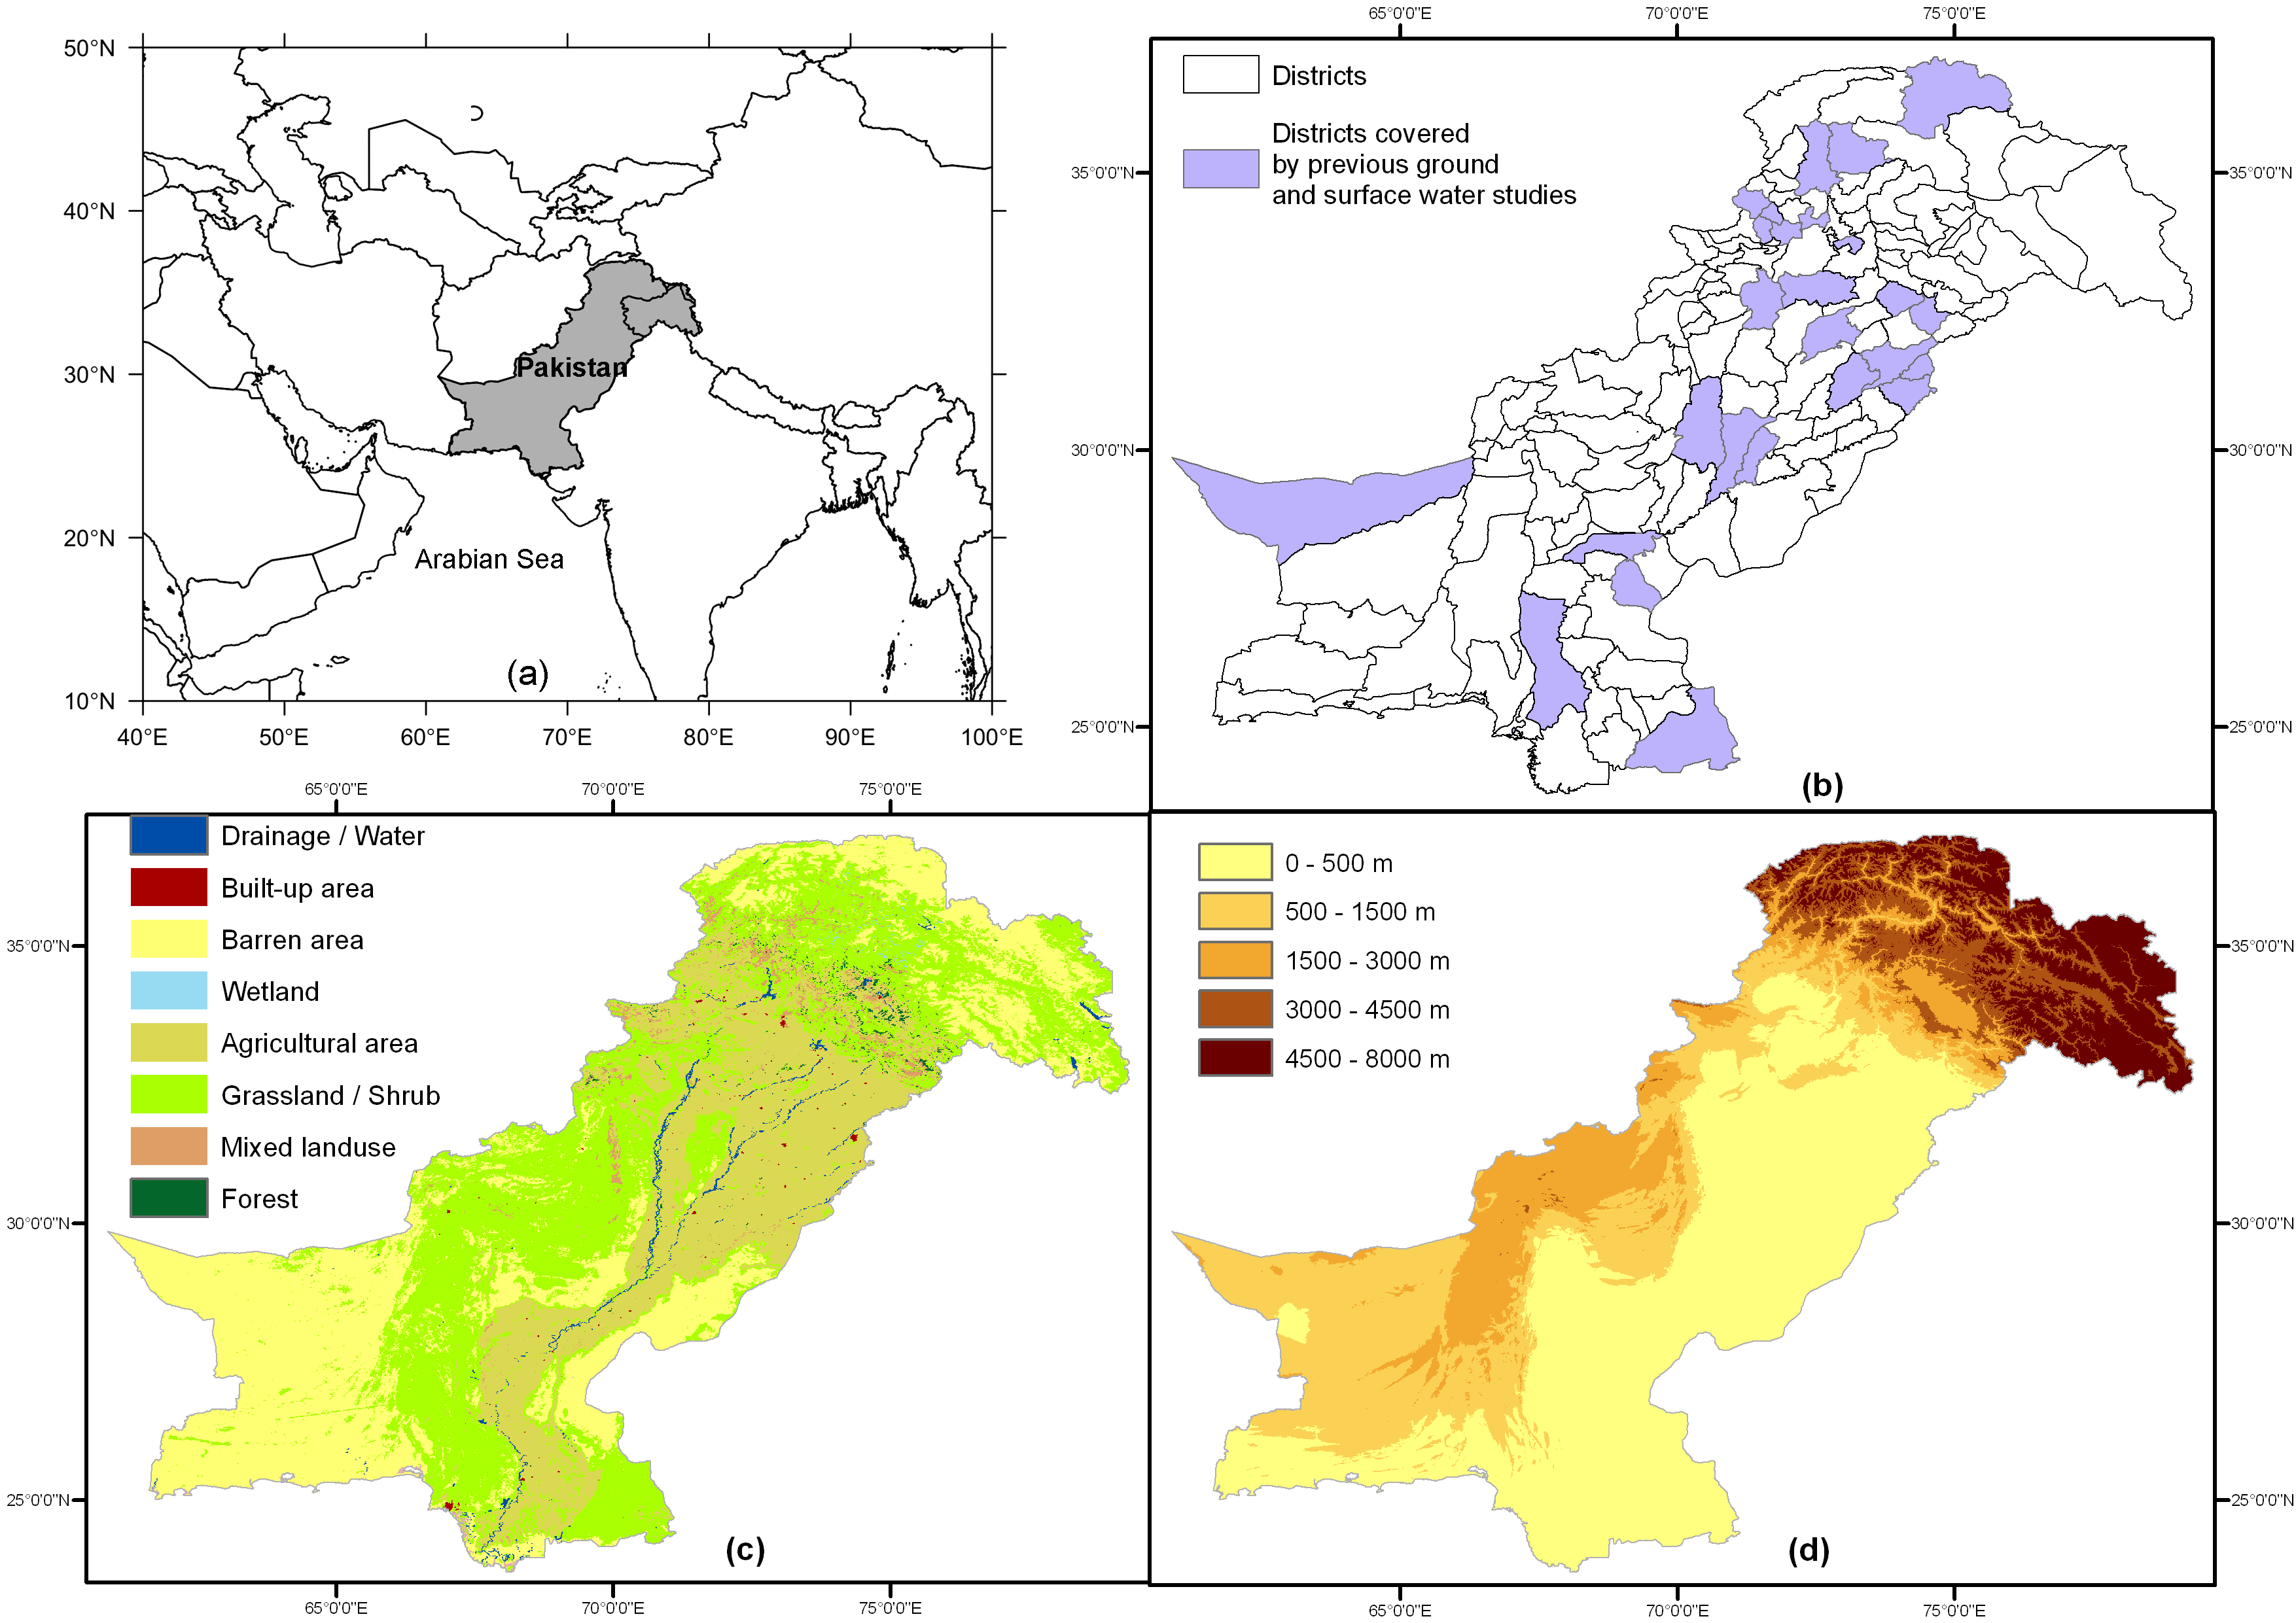
\includegraphics[width=\textwidth]{Figures/Fig_5_1.png}
  \caption{(a) Location of Pakistan in South Asia within the coastal belt of Arabian sea, (b) districts with available trace metal concentration for ground and surface water (see Table D.1 and D.2 in appendix D for details), (c) land cover map of Pakistan with the Indus river basin in the Eastern part of the country (ISCGM, 2014) and (d) elevation of Pakistan from mean sea level (Rodriguez et al., 2005).}
  \label{Fig_5_1}
\end{figure}

\subsection{Data compilation and processing}
\label{Data compilation and processing}

We compiled data on the concentrations of 10 trace metals, i.e. arsenic (As), cadmium (Cd), chromium (Cr), copper (Cu), iron (Fe), manganese (Mn), mercury (Hg), nickel (Ni), lead (Pb) and zinc (Zn) in ground and surface water of Pakistan, measured in multiple sites within 26 districts during 1991-2014, from previously published studies (Table D.1 and D.2 in appendix D). The individual studies provided concentration values that were typically corrected for sampling and processing errors (see cited studies in Table D.1 and D.2). In 82\% of the studies, concentration data were reported as summary statistics (e.g. mean, max and standard deviation, see Table D.1 and D.2 for details on the number of ground and surface water samples in each district used to compute the district mean) for the districts. The trace metal concentrations of samples from each district exhibited a low variation (all coefficient of variation (CV) $\leq$ 20\% and relative homogeneity of CV across districts) and no outlier value was detected in the data (cited studies in Table D.1 and D.2). Hence, given that in 96\% of the studies sampling sites were not geo-referenced, we regarded the mean as a sufficiently robust parameter and assigned district mean values to the georeferenced districts as the representative trace metal concentrations in the surface and ground water (country-level summary statistics are presented in Table D.3). In 5\% and 32\% of districts for ground and surface water, respectively, we had mean concentrations from two years for a few trace metals (Table D.1; D.2). In these cases, we used the latest concentrations to avoid heterogeneity in the uncertainty of predicted concentrations across trace metals and districts, and thus in risk assessment. The district level aggregation of trace metal concentrations may result in uncertainties regarding variability within the districts. However, given the large spatial extent of our study, i.e. country-level with 137 districts, we regarded information on the district-level variation as sufficient. Moreover, previous studies successfully predicted and analyzed the relationship of contaminants, diseases and other variables with their relevant drivers on similar or coarser spatial resolutions, e.g. counties (Videras, 2014), districts (Huang and Leung, 2002), and regions (Berke, 2004).

To identify the deviation in district-level trace metal concentrations from the country-level (global) mean and thus their global representativeness, we computed the global coefficient of variation (GCV) for each trace metal T (Eq. 5.1).

\begin{equation}
GCV_T=\frac{\sigma_T}{\mu_T}+100
\end{equation}

where, $\sigma_T$ and $\mu_T$ are the global standard deviation and mean of the district-level T trace metal concentrations, respectively.

Physical and chemical processes in surface and groundwater and sediment compositions are predominantly affected by adjacent soil properties and further geo-hydrological variables (e.g. soil type, depth of groundwater table, infiltration, seepage and climate), land use (e.g. industrial and agricultural) and different environmental variables (e.g. slope), and in turn these variables show strong correlations with trace metal concentrations (Huang et al., 2015; Pebesma and Kwaadsteniet, 1997; Rodríguez-Lado et al., 2013). Hence, we compiled raster data on the soil properties (also as surrogates of geo-hydrological variables because they are presumably correlated), land cover and elevation (surrogate of environmental variables) for Pakistan. Soil properties data with 0.5 degrees (\textasciitilde 55.5 km) resolution, land cover data with 0.008 degrees (\textasciitilde 925 m) resolution and elevation data with 90 m resolution were obtained from the global soil properties dataset (Batjes, 2000), the Global Map of Pakistan: version 1.1 (ISCGM, 2014) and the digital elevation model (DEM) from Shuttle Radar Topography Mission (SRTM) (Rodriguez et al., 2005), respectively. The data were cropped to the spatial extent of Pakistan and transformed to the WGS 1984 coordinate reference system. The soil properties and land cover data initially included six and eight variables, respectively (Batjes, 2000; ISCGM, 2014). From all raster cells within each district with trace metal concentration data (sampled), the mean soil properties and percentages of different land covers were computed and checked for their spatial correlation with trace metal concentrations. The four soil property variables, i.e. total available water capacity (WC, mm water per 1 m soil depth), soil organic carbon density (SOC, kg C/m\textsuperscript{2} for 0-100 cm depth range), soil carbonates carbon density (SCC, kg C/m\textsuperscript{2} for 0-100 cm depth range) and soil pH (30-100 cm depth range), and the three land cover variables, i.e. \% built-up area (BLU), \% agricultural area (ALU) and \% mixed land use (MLU) area that showed statistically significant correlation with at least one trace metal concentration were included in the final analysis. For these subsetted variables, we extracted the means (for soil property variables) and percentages (for land cover variables) from the rasters also for the districts without trace metal concentrations (unsampled). In addition, the mean elevation (ELV) was calculated per district. Finally, we collected population data for Pakistani districts from the Pakistan Bureau of Statistics (2010). Spatial transformation and extraction of spatial predictor variables was performed using the “maptools” (Lewin-Koh et al., 2011) and “raster” (Hijman and Van Etten, 2010) packages in R (R Core Team, 2014).

\subsection{Spatial prediction of trace metal concentrations in ground and surface water}
\label{Spatial prediction of trace metal concentrations in ground and surface water}

The geographically weighted regression (GWR) model was applied for spatial prediction of the trace metal concentrations in the ground and surface water, separately, at unsampled districts fitted with selected spatial predictors (Fotheringham et al., 2002; Harris et al., 2010). District level trace metal concentrations showed a high dispersion from the global mean (GCV $>$ 1) and hence indicated a low global representativeness (Table D.3). Moreover, only a few districts were sampled by the previous studies resulting in a low sample density and thus large distances between the districts (Figure 5.1; Table D.3). Hence, the GWR model was chosen because it allows to incorporate local variations of the trace metal concentrations with respect to spatial auto-correlation and non-stationarity in the model parameters (Fotheringham et al., 2002; Harris et al., 2010). Moreover, compared to global spatial prediction techniques such as kriging, the GWR has been shown to better represent the spatially varying relationship between water quality parameters and different spatial predictors (Javi et al., 2014; Huang et al., 2015; Tu and Xia, 2008). Furthermore, GWR allowed for modelling spatial variability of trace metals at district level resolution with low uncertainty (Lin et al., 2011). A GWR model was calibrated for the concentration of each trace metal $T$ in ground and surface water for the sampled districts $z$ by evaluating the local relationship between trace metal concentration $C_{T,z}$ and spatial predictors $S$ (Eq. 5.2).

\begin{equation}
C_{T,z}=\delta_{z,0}+\displaystyle\sum_{n=1}^{m=8}\delta_{z,n}S_{z,n}+e_z
\end{equation}

where $S_{z,n}$ is the value of the $n$th spatial predictor (={WC, SOC, SCC, pH, BLU, ALU, MLU and ELV}), $m$ is the number of spatial predictors (=8), $\delta_{z,0}$ is the intercept parameter, $\delta_{z,n}$ is the local regression coefficient for the $n$th spatial predictor and $e_z$ is the random error. The GWR model estimates the local regression coefficients for the spatial predictors using a moving window technique and a weighted least square approach (Figure D.1). The weights are obtained using a distance-decay kernel function among the centroids of neighboring sampled districts. We chose a “gaussian” kernel, based on the assumption of spatial continuity of the trace metal concentration in ground and surface water, as the water bodies are connected through a network within the Indus river delta (Harris et al., 2010; Pakistan Bureau of Statistics, 2010). The size of the moving window (great circle distances between district centroids in our case) is controlled by a kernel bandwidth that was selected using the Akaike Information Criterion corrected for small sample sizes (AICc) (Table 5.1) (Akaike, 1973). For each trace metal, the best-fit GWR model was identified by forward entering of the eight spatial predictors and using the AICc values as goodness of fit criterion. The best-fit model (minimal AICc) was selected for prediction of each of the trace metals in ground and surface water, separately, in unsampled districts (Figure 5.2; 5.3). Spatial prediction for Hg in ground water was omitted because of the very small sample size (n= 2) (Table D.3). GWR model selection, calibration and the spatial prediction were performed using the “GWmodel” package (Gollini et al., 2013) in R (R Core Team, 2014).

\subsection{GWR model validation}
\label{GWR model validation}

We evaluated the spatial prediction quality of the GWR models in terms of prediction accuracy and the agreement between model predicted and observed concentrations (Gollini et al., 2013). To predict the accuracy, the observed concentrations of a district were compared to the concentrations

\begin{landscape}

\begin{table}[h]

\label{Table 5.1}

\caption{Calibrated geographically weighted regression (GWR) models and their spatial prediction quality for the concentration of trace metals in ground and surface water of unsampled districts. Corresponding corrected Akaike Information Criterion (AICc), kernel bandwith (size of the moving window), root mean square deviation error (RMSDE), index of agreement ($d$), mean (MZ) and standard deviation (SDZ) of the prediction z-scores are provided.}

\begin{threeparttable}
\centering

\begin{tabular}{>{\centering\arraybackslash}m{2.0cm}>{\centering\arraybackslash}m{2.0cm}>{\centering\arraybackslash}m{3.0cm}>{\centering\arraybackslash}m{1.5cm}>{\centering\arraybackslash}m{4.0cm}>{\centering\arraybackslash}m{0.7cm}>{\centering\arraybackslash}m{0.7cm}>{\centering\arraybackslash}m{1.0cm}>{\centering\arraybackslash}m{0.7cm}}

\toprule
\multirow{2}{2.0cm}{\centering\textbf{Trace metal}} & \multirow{2}{2.0cm}{\centering\textbf{Source}} & \multirow{2}{3.0cm}{\centering\textbf{Selected GWR model}} & \multirow{2}{1.5cm}{\centering\textbf{AICc}} & \multirow{2}{4.0cm}{\centering\textbf{Kernel bandwith (great circle distance between district centroids, km)}} & \multicolumn{2}{c}{\centering\textbf{Prediction quality}} & \multicolumn{2}{c}{\centering\textbf{Prediction uncertainty}}\\
 & & & & & \textbf{RMSDE} & \textbf{$d$} & \textbf{MZ} & \textbf{SDZ}\\
 & & & & & & & & \\

\midrule

\multirow{2}{2.0cm}{\centering As} & Ground water & As\textunderscore GW \textasciitilde SOC & 13.46 & 1104.30 & 0.27 & 0.67 & -0.01 & 0.77\\
 & Surface water & As\textunderscore SW \textasciitilde SOC+pH & -1255.80 & 521.98 & 0.08 & 0.97 & -0.06 & 0.22\\
\multirow{2}{2.0cm}{\centering Cd} & Ground water & Cd\textunderscore GW\textasciitilde SOC+SCC & -9140.39 & 1299.72 & 0.06 & 0.90 & -0.10 & 0.13\\
 & Surface water & Cd\textunderscore SW\textasciitilde ALU & -29.10 & 1321.05 & 0.04 & 0.79 & -0.01 & 0.69\\
\multirow{2}{2.0cm}{\centering Cr} & Ground water & Cr\textunderscore GW\textasciitilde BLU & -21.27 & 500.64 & 0.06 & 0.99 & 0.00 & 0.77\\
 & Surface water & Cr\textunderscore SW\textasciitilde WC+ALU & -4014.42 & 1321.14 & 0.04 & 0.92 & -0.05 & 0.21\\
\multirow{2}{2.0cm}{\centering Cu} & Ground water & Cu\textunderscore GW\textasciitilde SOC & 33.75 & 1299.58 & 0.61 & 0.43 & 0.00 & 0.75\\
 & Surface water & Cu\textunderscore SW\textasciitilde WC & -31.45 & 1321.05 & 0.04 & 0.79 & -0.03 & 0.74\\
\multirow{2}{2.0cm}{\centering Fe} & Ground water & Fe\textunderscore GW\textasciitilde WC & 43.33 & 1147.75 & 0.97 & 0.39 & 0.02 & 0.77\\
 & Surface water & Fe\textunderscore SW\textasciitilde SOC & 45.45 & 1320.77 & 0.95 & 0.44 & 0.00 & 0.78\\
\multirow{2}{2.0cm}{\centering Mn} & Ground water & Mn\textunderscore GW\textasciitilde SCC+BLU & -9764.11 & 1299.72 & 0.22 & 0.95 & -0.06 & 0.14\\
 & Surface water & Mn\textunderscore SW\textasciitilde WC+ALU & -3675.37 & 1321.14 & 0.07 & 0.86 & -0.05 & 0.20\\
Hg & Surface water & Hg\textunderscore SW\textasciitilde SCC+BLU & -1543.69 & 453.07 & 0.02 & 0.98 & -0.06 & 0.30\\
\multirow{2}{2.0cm}{\centering Ni} & Ground water & Ni\textunderscore GW\textasciitilde SCC & 22.88 & 1299.36 & 0.42 & 0.51 & -0.03 & 0.78\\
 & Surface water & Ni\textunderscore SW\textasciitilde WC & -29.23 & 1335.07 & 0.04 & 0.88 & -0.02 & 0.70\\
\multirow{2}{2.0cm}{\centering Pb} & Ground water & Pb\textunderscore GW\textasciitilde BLU & 8.52 & 1299.49 & 0.21 & 0.96 & -0.02 & 0.78\\
 & Surface water & Pb\textunderscore SW\textasciitilde ALU & -18.70 & 1321.00 & 0.07 & 0.75 & 0.01 & 0.75\\
\multirow{2}{2.0cm}{\centering Zn} & Ground water & Zn\textunderscore GW\textasciitilde BLU & 26.64 & 1299.36 & 0.45 & 0.95 & 0.01 & 0.80\\
 & Surface water & Zn\textunderscore SW\textasciitilde SOC & 42.63 & 1335.07 & 0.80 & 0.31 & -0.01 & 0.79\\

\bottomrule

\end{tabular}

\begin{tablenotes}
\footnotesize
As = Arsenic, Cd = Cadmium, Cr = Chromium, Cu = Copper, Fe = Iron, Mn = Manganese, Hg = Mercury, Nickel = Ni, Pb = Lead, Zn = Zinc,  GW = ground water, SW = surface water, WC = mean total available water capacity, SOC = mean soil organic carbon density, SCC = mean soil carbonate carbon density, pH= mean soil pH, BLU = percentage of built-up area, ALU = percentage of agricultural area.
\end{tablenotes}

\end{threeparttable}

\end{table}

\end{landscape}

\noindent predicted for this district using the respective GWR model in terms of root mean squared deviation error (RMSDE) (Eq. 5.3) computed through a leave-one-out cross validation (see Gollini et al. (2013) for details). Similarly, the index of agreement ($d$) was computed to quantify the agreement between GWR model predicted and observed trace metal ($T$) concentrations (Eq. 5.4) (Table 5.1) (Willmott, 1984).

\begin{equation}
RMSDE_T=\displaystyle\sum_{z=1}^{n}\sqrt{\frac{1}{n}(P_{T,z}-O_{T,z})^2}
\end{equation}

\begin{equation}
d_T=1-\frac{n*RMSDE_T^2}{\displaystyle\sum_{z=1}^{n}(|P_{T,z}-\bar{O}_T|+|O_{T,z}-\bar{O}_T|)^2}
\end{equation}

where, $RMSDE_T$ and $d_T$ are the RMSDE and $d$ for the GWR model predictions, $P_{T,z}$ and $O_{T,z}$ are model predicted and observed concentration values in district $z$, $n$ is the number of districts and $\bar{O}_T$ is the mean of the observed district level concentrations. The RMSDE should tend to zero to indicate the accurate prediction of GWR. The $d$ values vary on a scale from 0 to 1, 0 indicating no agreement and 1 the perfect agreement. GWR model validation was performed using the “GWmodel” (Gollini et al., 2013) and “hydroGOF” (Zambrano-Bigiarini, 2014) packages in R (R Core Team, 2014).

\subsection{GWR prediction uncertainties}
\label{GWR prediction uncertainties}

We computed nationwide (global) GWR prediction uncertainties for trace metal concentrations in ground and surface water by the mean (MZ) standard deviation (SDZ) of the prediction z-scores (Table 5.1) (Gollini et al., 2013).  Zero MZ and the unity of SDZ indicate high certainty in the prediction by GWR. In a second step, we calculated standard error maps for predictions of trace metal concentrations in ground and surface water to investigate the GWR model prediction uncertainties for each district (local) (Figure D.2). Finally, we computed ranges in the GWR model predicted trace metal concentration values within 95\% confidence interval based on local prediction uncertainties, i.e. GWR predicted values $\pm$ 1.96 * standard errors (Figure D.3; D.4). GWR prediction uncertainty was computed using the “GWmodel” package (Gollini et al., 2013) in R (R Core Team, 2014).

\subsection{Risk prediction}
\label{Risk prediction}

We computed a human health risk quotient (RQ) for each trace metal concentration to predict their exceedances of threshold concentrations in each district (Törnqvist et al., 2011) (Eq. 5.5).

\begin{equation}
RQ_{T,z}=\frac{\hat{C}_{T,z}}{C_{WHO-T}}
\end{equation}

where, for the $T$th trace metal in ground or surface water at district $z$, $\hat{C}_{T,z}$ is the estimated concentration by GWR and $C_{WHO-T}$ is the threshold concentration derived by the World Health Organization (WHO guideline values based on human health targets) for drinking water for the trace metal T (WHO, 2011). In the absence of WHO values for Fe, we used the criteria guidelines values from the environmental protection agency (EPA)-Pakistan (Azizullah et al., 2011). A RQ $\leq$ 1 indicates negligible risk (lower- than or equal concentration to the WHO guideline value), whereas RQ $>$ 1 indicates a health risk (higher concentration than the WHO guideline value) to the consumers from drinking contaminated water (Törnqvist et al., 2011) and, accordingly, the risk related to ground and surface waters for a district was mapped (Figure 5.4; 5.5). Finally, the proportion of total area of Pakistan at risk and total inhabitants in risky districts were calculated through a spatial overlay of the created risk maps with district area and population data (Table 5.2).

\subsection{Risk prediction uncertainties}
\label{Risk prediction uncertainties}

To address the uncertainties in risk prediction, we computed RQ values for the lower and upper confidence boundaries (CB) of predicted trace metal concentrations, i.e. GWR predicted values $\pm$ 1.96 * standard errors (Figure D.5; D.6). The proportion of total area at risk and total inhabitants in risky districts were also computed for the lower and upper CB of predicted trace metal concentrations (Table 5.2).

\begin{figure}[t]
  \centering
  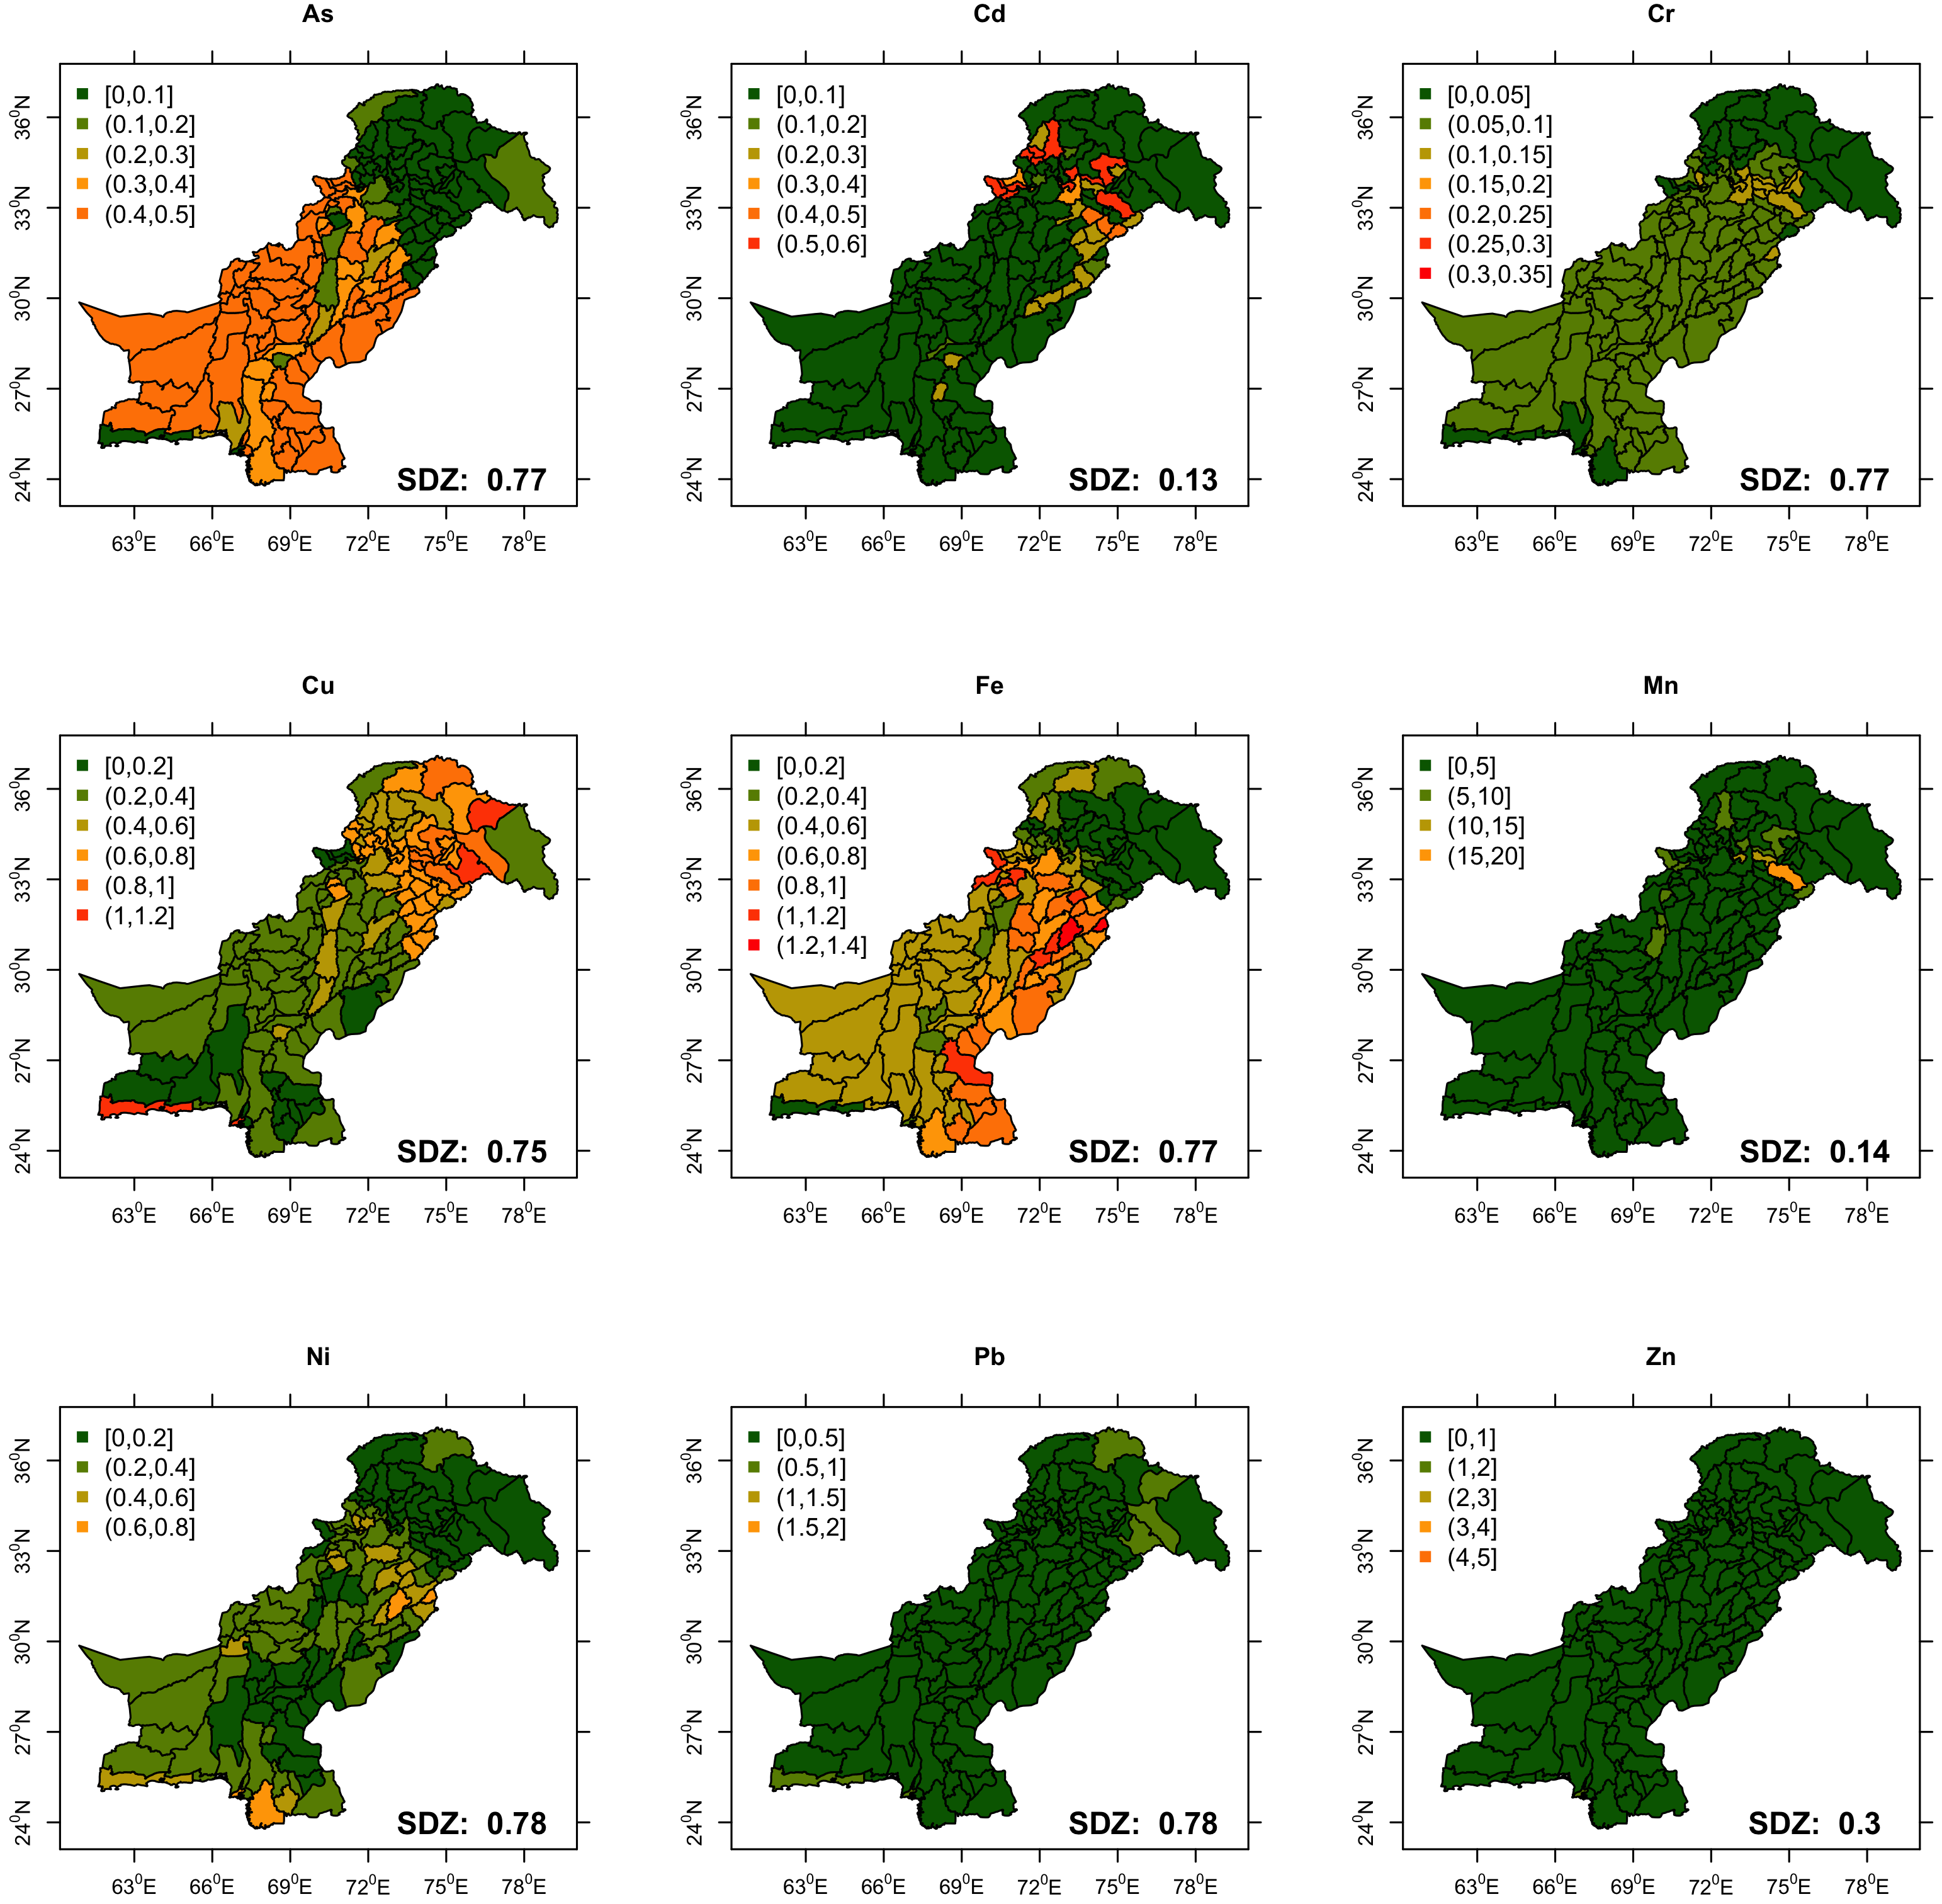
\includegraphics[width=\textwidth]{Figures/Fig_5_2.png}
  \caption{Geographically weighted regression predicted concentration values in mg/l (see legend) of the trace metals in ground water at the districts of Pakistan.  The abbreviations used: As = Arsenic, Cd = Cadmium, Cr = Chromium, Cu = Copper, Fe = Iron, Mn = Manganese, Nickel = Ni, Pb = Lead, Zn = Zinc.}
  \label{Fig_5_2}
\end{figure}

\begin{landscape}
\begin{figure}[t]
  \centering
  \vspace*{-1.5cm}
  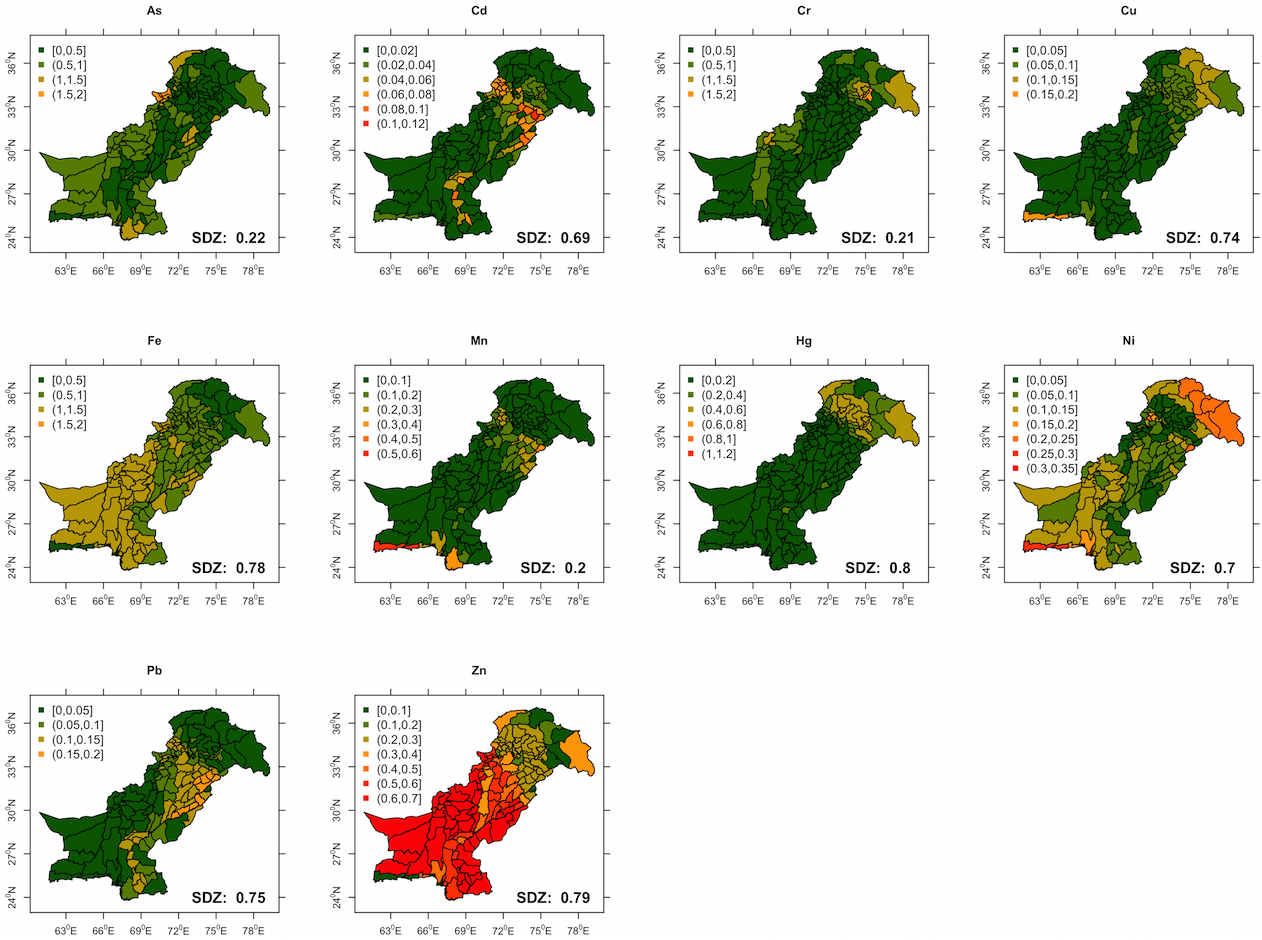
\includegraphics[width=0.9\linewidth]{Figures/Fig_5_3.png}
  \caption{Geographically weighted regression predicted concentration values values in mg/l (see legend) of the trace metals in surface water at the districts of Pakistan.  The abbreviations used: As = Arsenic, Cd = Cadmium, Cr = Chromium, Cu = Copper, Fe = Iron, Mn = Manganese, Hg = Mercury, Nickel = Ni, Pb = Lead, Zn = Zinc.}
  \label{Fig_5_3}
\end{figure}
\end{landscape}

\begin{figure}[t]
  \centering
  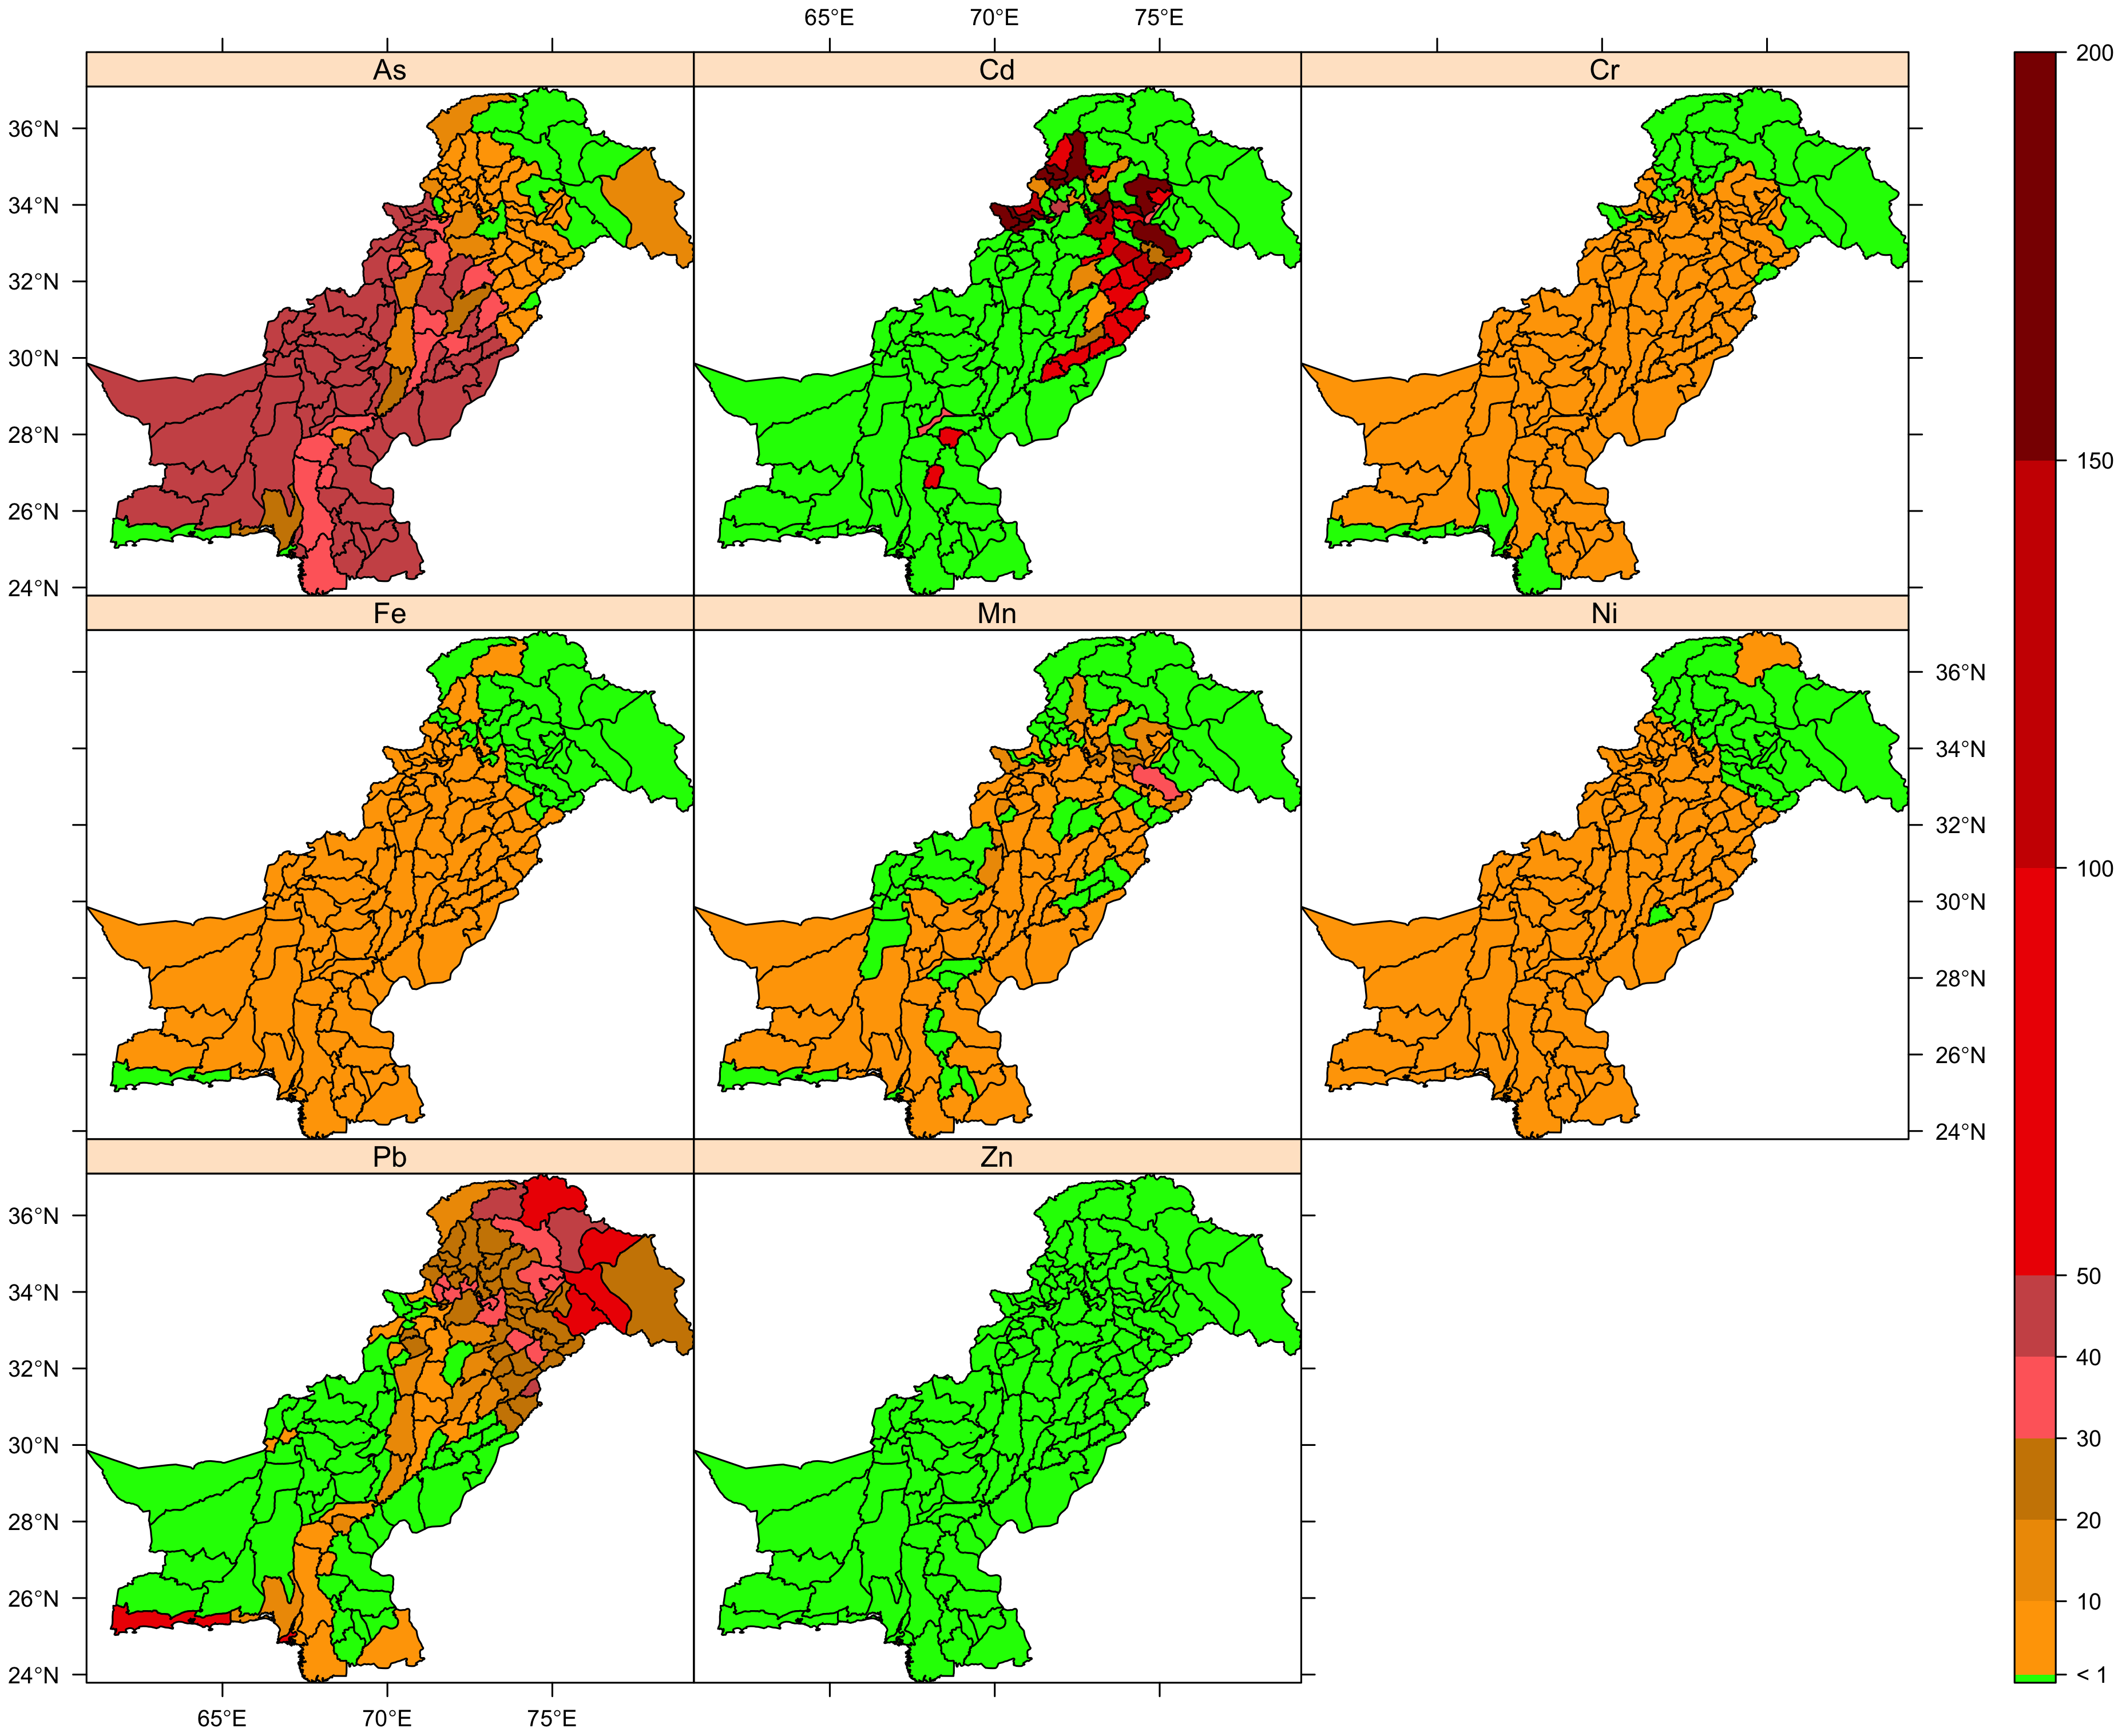
\includegraphics[width=\textwidth]{Figures/Fig_5_4.png}
  \caption{Predicted risks, i.e. exceedances of threshold concentrations in risk quotients (RQ), for the districts of Pakistan from predicted concentrations of trace metals in the ground water. Green indicates no exceedance, i.e. RQ $\leq$ 1. The abbreviations used: As = Arsenic, Cd = Cadmium, Cr = Chromium, Cu = Copper, Fe = Iron, Mn = Manganese, Nickel = Ni, Pb = Lead, Zn = Zinc. Map of Cu is omitted because no risky district was found, i.e. for none of the district RQ $>$ 1.}
  \label{Fig_5_4}
\end{figure}

\begin{figure}[t]
  \centering
  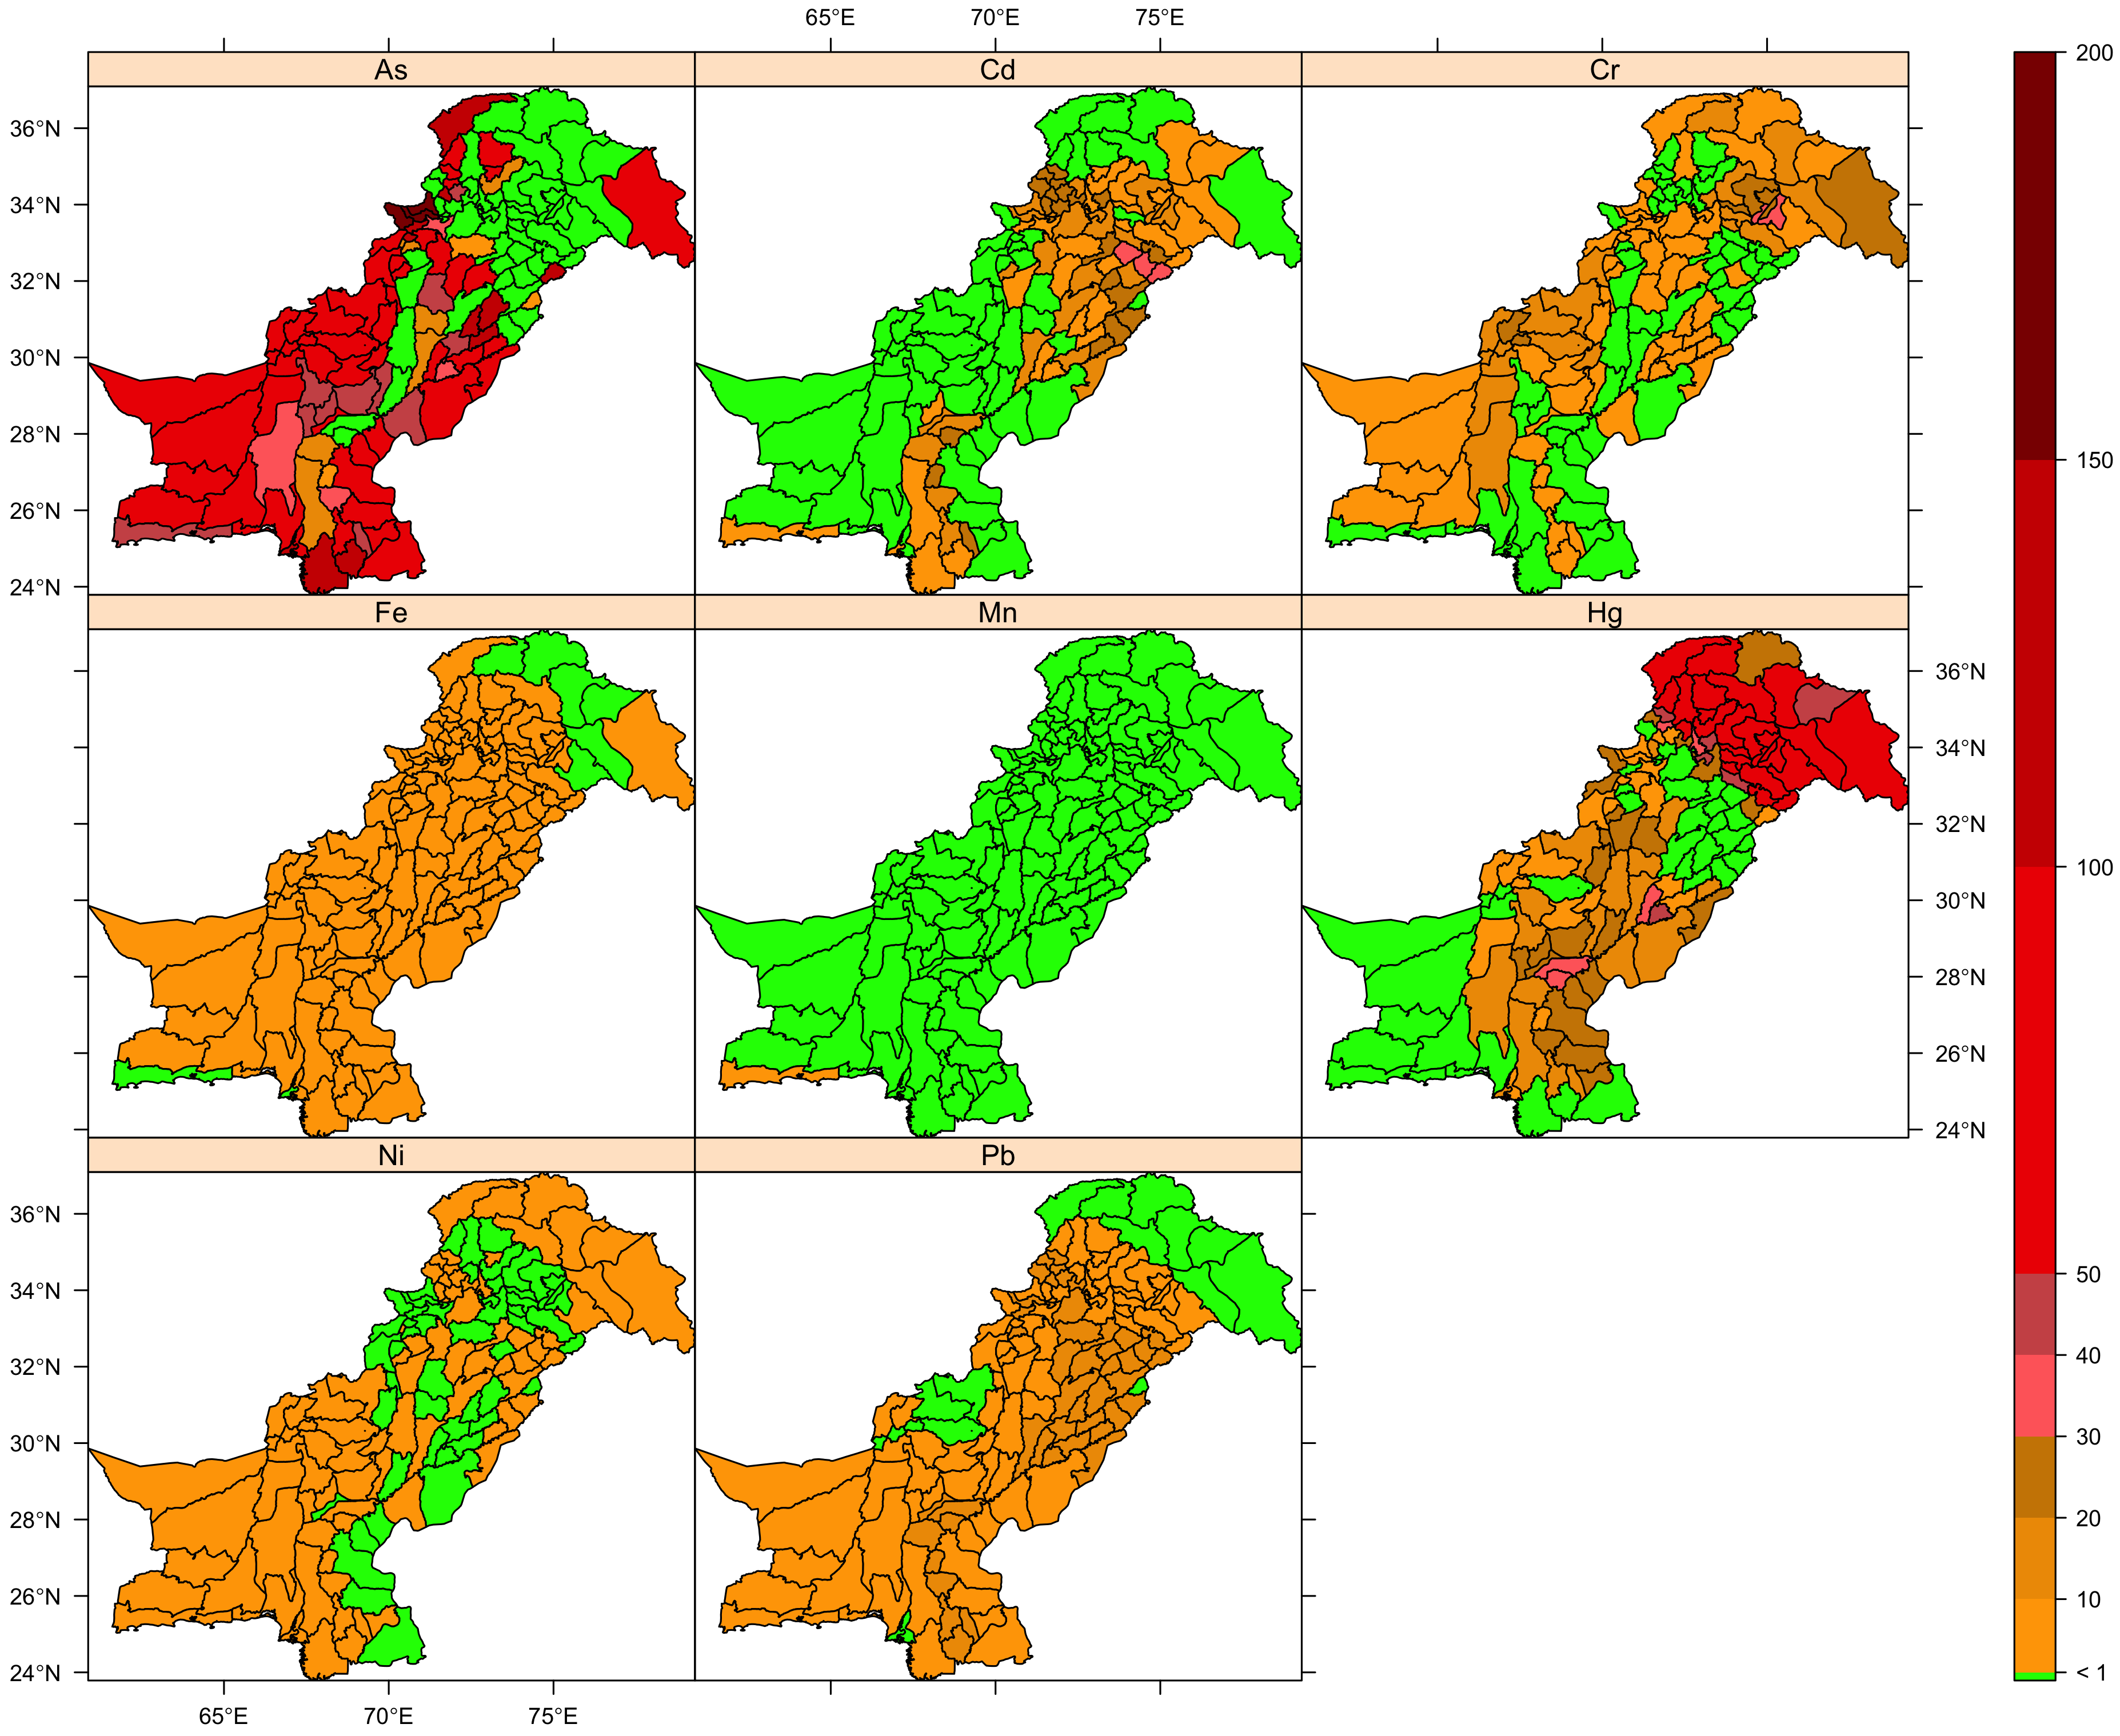
\includegraphics[width=\textwidth]{Figures/Fig_5_5.png}
  \caption{Predicted risks, i.e. exceedances of threshold concentrations in risk quotients (RQ), for the districts of Pakistan from predicted concentrations of trace metals in the surface water. Green indicates no exceedance, i.e. RQ $\leq$ 1. The abbreviations used: As = Arsenic, Cd = Cadmium, Cr = Chromium, Cu = Copper, Fe = Iron, Mn = Manganese, Hg = Mercury, Nickel = Ni, Pb = Lead, Zn = Zinc. Maps of Cu and Zn are omitted because no risky district was found, i.e. for none of the district RQ $>$ 1.}
  \label{Fig_5_5}
\end{figure}

\section{Results and Discussion}
\label{Results and Discussion}

\subsection{GWR prediction of trace metal concentration in ground and surface water}
\label{GWR prediction of trace metal concentration in ground and surface water}

We predicted the concentrations of 10 trace metals in surface and ground water of Pakistan by using the best-fit GWR models with selected spatial predictors. Out of eight spatial predictors that were selected based on statistically significant correlations in a preliminary analysis, six predictors were included in the best-fit GWR models based on the AICc (Table 5.1). Soil properties variables, i.e. WC, SOC, SCC, and pH, which represent a surrogate of geo-hydrological variables, were the spatial predictors of As, Fe and Ni. The As, Fe and Ni contamination of drinking water sources in Pakistan can largely be attributed to the natural geogenic sources that are causally related to the soil properties and geo-hydrology (Azizullah et al., 2011; Shah et al., 2012). For example, As contamination of ground water in many parts of Pakistan results from the presence of Holocene sediments brought by alluvial deposits into arid to semi-arid zones and the subsequent As release due to As-desorption in oxic aquifers (Amini et al., 2008; Farooqi et al., 2008). Moreover, the ground as well as surface water sediments are rich in “micas” dominated by “biotite” mineral that contains As and releases As under high pH level (Husain et al., 2012). Furthermore, surface water from the Himalayas erodes As-rich sediments resulting in elevated As levels in downstream areas (Husain et al., 2012). By contrast, agricultural (ALU) and built-up (BLU) land covers were the dominant predictors of Cr, Hg and Pb concentrations in ground and surface waters. Agricultural and built-up land covers indicate anthropogenic input of trace metals, e.g. via industrial point discharge and runoff from agricultural and impervious urban surfaces. The source of Cr input has been attributed to the discharge of effluents from leather industries, which use Cr-salts for leather tanning (Farooqi et al., 2008; Baig et al., 2009). Pb contamination is largely associated with the manufacturing of electrical appliances, uncontrolled discharge from chemical industries and pesticide runoff (Tariq et al., 1996; Abdullah et al., 2015). Hg in surface water may originate from the traditional practice of amalgamation and smelting in gold panning activities (Ashraf et al., 1991). Moreover, cement manufacturing, coal mining and disposal of untreated municipal and hospital wastes into streams have been suggested as main causes of Hg contamination in the East and Southeast of Pakistan (Malkani, 2012; Kalhoro et al., 2014). Thus, the spatial predictors selected in our study are in agreement with the causes of trace metal contamination identified in previous studies. Inclusion of more relevant predictors, i.e. properties of river- and lake-bed sediments, chemical composition of aquatic environment and industrial discharge and pesticide runoff in the catchments might enhance the robustness of our results (Huang et al., 2015; Rodríguez-Lado et al., 2013), though such data are currently unavailable for Pakistan.

The selected spatial predictors exhibited stronger relationship with the concentrations of most trace metals, i.e. higher local GWR coefficients, for the districts in the North than the South of Pakistan (Figure D.1). For example, Cd concentration in ground and surface water exhibited stronger relationship with SCC, SOC and ALU, respectively, for the districts in the North than the South. High Cd contamination of ground water in the northern mountainous districts of Pakistan were attributed to rock phosphates that leach into aquifer whereas Cd contamination of surface water in the northern agricultural zones were related to chemical fertilizers (Abdullah et al., 2014). However, As, Mn and Zn concentration in ground and surface water showed stronger relationship with the predictors in the South than the North (Figure D.1). Overall, spatial predictors representing geogenic sources (WC, SOC, SCC and pH) showed stronger relationship with trace metal concentrations than the predictors representing anthropogenic input (ALU and BLU) for all districts in Pakistan (Figure D.1). Hence, geogenic processes may be more important than anthropogenic inputs for trace metal contamination in ground and surface water of Pakistan.

The GWR model predictions exhibited a good (d $\geq$ 0.8) agreement with the observed concentrations and relatively high prediction accuracy (RMSDE $\leq$ 0.22) for most of the trace metals independent of the number of sampled districts (Table 5.1; D.3). However, the prediction for Fe in ground water and Zn in surface water exhibited a relatively low (d $<$ 0.4) agreement with observed concentrations, which coincided with a lower prediction accuracy, i.e. RMSDE = 0.97 and 0.80 for Fe and Zn, respectively. The low goodness of fit for Fe and Zn may be explained by their high spatial variation (GCV $>$ 1.9) (Table D.3).  The highest prediction accuracy and agreement were obtained for Hg despite of only seven sampled districts (Table 5.1). Nevertheless, the predicted risk maps should be interpreted with caution irrespective of the model metrics, because of the small sample size and low global representativeness, and thus the high goodness-of-fit may only correspond to a few sampled and neighboring districts.

In general, the prediction of trace metal concentrations exhibited a low global uncertainty (-0.03 $\geq$ MZ $\geq$ 0.02 and SDZ $\geq$ 0.7) (Table 5.1). However, prediction of a few trace metals, i.e. Cd in ground water, As and Cr in surface water and Mn in both ground and surface water showed a high uncertainty (MZ $\leq$ -0.05 and SDZ $\leq$ 0.3). Spatial prediction for Cd in ground water and Mn in surface water exhibited the highest uncertainty (MZ $\leq$ -0.06 and SDZ $\leq$ 0.14) and hence, the predicted values for these metals should be regarded with caution.

Higher prediction standard errors and thus higher local prediction uncertainties were obtained for the Northeastern mountainous districts and southern coastal districts than for central parts of Pakistan (Figure D.2). This may be attributed to data scarcity in terms of lowest density of sampled districts in these regions (Figure 5.1b). Hence, predictions for these districts should be interpreted with caution. In all districts, predictions for Fe in ground water and Zn in surface water exhibited higher standard errors than other trace metals, which is in line with the overall lower agreement and accuracy of predictions for these trace metals. Predictions for Mn in both surface and ground water showed high standard error for all districts, particularly for the districts in the South (Figure D.2). Overall, prediction accuracy of trace metal concentrations decreased with increasing distance to the sampled districts (Figure 5.1b; D.2).

The calibrated kernel bandwidths (size of the moving window) that indicate the maximum great circle distances between the centroids of unsampled and sampled districts in GWR model predictions were between 450 km and 1300 km (Table 5.1). This indicates a low density of trace metal samples, i.e. the unsampled districts are at a large distance from sampled districts, especially for the bandwidths $\geq$ 1000 km. Thus, the predictions for the unsampled districts may not reflect the true variation of trace metal concentration between sampled and unsampled districts (Bhowmik and Costa, 2014; Goovaerts, 1997). However, GWR models incorporate local variation in the regional scale prediction by defining local models for each prediction location and weight local regression coefficients based on the distances from neighboring observations. Thus, if all samples are at large distances from the prediction location, they have a low influence in prediction and local spatial predictors mainly determine trace metal concentration, and hence GWR results in high accuracy by reducing under- and overestimation (Fotheringham et al., 2002; Gollini et al., 2013; Harris et al., 2010). Thus, we suggest that our model predictions are sufficiently robust, though a more thorough validation would require data from field monitoring.

Our GWR model predicted concentrations (Figure 5.2; 5.3) as well as the lower and upper confidence boundaries (CB) (Figure D.3; D.4) generally showed higher values in Northern and Southern districts than central districts for all studied trace metals. The predicted concentrations of Cr and Ni in the mountainous Northeast and flat Southwest (Figure 5.1) of the country showed four fold higher values than in other parts. High Pb-contaminated districts are primarily located in the mountainous Northeast of Pakistan with two fold higher concentrations than in other parts of the country (Figure D.3; D.4). Moreover, high Hg contamination was predicted for surface waters of most districts with particularly high levels (four fold higher than the South) in the mountainous North. In general, districts with a high concentration of a trace metal in surface water also exhibited a high concentration of that metal in ground water (Figure 5.2; 5.3). Therefore, Hg concentrations in the ground water of districts with high concentrations in the surface water may also be elevated. However, this could not be evaluated due to a lack of measurements and hence we recommend the inclusion of Hg in future ground water monitoring of Pakistan.

\subsection{Human health risk from trace metals}
\label{Human health risk from trace metals}

The nationwide approximated risk maps indicate that predicted concentrations of most trace metals exceeded WHO drinking water threshold values (RQ $>$ 1) and thus indicated human health risks for Pakistan (Figure 5.4; 5.5). Risk prediction for the lower CB of predicted concentrations also indicated an exceedance of WHO thresholds by most trace metals, where for the upper CB thresholds were exceeded by all trace metals except for Cu (Figure D.5; D.6). The highest exceedance was observed for As and Cd, where in ground water their exceedances were 40-50 and 150-200 fold, and in surface water 150-200 and 30-40 fold, respectively (Figure 5.4; 5.5). The exceedances observed for the lower CB of predicted As and Cd concentrations were 10-20 and 20-30 fold, and 50-100 and 20-30 fold in ground and surface water, respectively. For the upper CB of As and Cd concentrations, the exceedances were 50-100 and 150-200 fold, and 150-200 and 100-150 fold in ground and surface water, respectively (Figure D.5; D.6). Predicted concentrations of Pb as well as their upper CB in ground water exceeded WHO thresholds by 50-100 times for the northern mountainous and southern coastal districts, whereas for the lower CB the exceedances were 20-30 fold (Figure 5.4; D.5; D.6). Predicted Hg concentrations as well as their lower and upper CB in surface water also exhibited an exceedance of 50-100 fold for the Northern districts (Figure 5.4; D.5; D.6). Cr, Fe, Mn and Ni showed maximum exceedances of 30-40 fold, especially for the Southern districts (Figure 5.4; 5.5). However, for the lower and upper CB of predicted concentrations they exceeded WHO thresholds by 10-20 and 40-50 times, respectively, in surface water (Figure D.6). Overall, health risks increase with exceedances of the thresholds for the trace metals, and hence districts with high exceedances should be prioritized in risk mitigations. However, note that the exceedances should be compared between districts and not between trace metals, because the dose-response relationships most likely differ.

\begin{table}[h]
\label{Table 5.2}
\caption{Estimated percentage of area and total population (million) at risk from trace metals in ground and surface water of Pakistan.}
\centering

\begin{threeparttable}
\centering

\begin{tabular}{>{\centering\arraybackslash}m{1.0cm}>{\centering\arraybackslash}m{2.0cm}>{\centering\arraybackslash}m{1.0cm}>{\centering\arraybackslash}m{1.2cm}>{\centering\arraybackslash}m{1.0cm}>{\centering\arraybackslash}m{1.2cm}>{\centering\arraybackslash}m{1.0cm}>{\centering\arraybackslash}m{1.2cm}}

\toprule
\textbf{Trace metal} & \textbf{Source} & \multicolumn{2}{c}{\centering\textbf{Predicted concentrations}} & \multicolumn{2}{c}{\centering\textbf{Lower CB}} &  \multicolumn{2}{c}{\centering\textbf{Upper CB}}\\
 & & \textbf{Area at risk} & \textbf{Population at risk} & \textbf{Area at risk} & \textbf{Population at risk} & \textbf{Area at risk} & \textbf{Population at risk}\\
 & & \textbf{(\%)} & \textbf{(million)} & \textbf{(\%)} & \textbf{(million)} & \textbf{(\%)} & \textbf{(million)}\\

\midrule

\multirow{2}{As} & Ground water & 86.60 & 156.7 & 56.07 & 63.05 & 100 & 172.30\\
 & Surface water & 73.40 & 120.9 & 65.91 & 75.24 & 100 & 172.30\\
\multirow{2}{Cd} & Ground water & 14.30 & 84 & 4.19 & 20.92 & 100 & 172.30\\
 & Surface water & 37.00 & 127.3 & 7.75 & 41.69 & 100 & 172.30\\
\multirow{2}{Cr} & Ground water & 74.70 & 160 & 0.02 & 23.50 & 100 & 172.30\\
 & Surface water & 68.70 & 74.1 & 29.61 & 12.94 & 100 & 172.30\\
\multirow{2}{Cu} & Ground water & 0 & 0 & 0 & 0 & 5.96 & 0.33\\
 & Surface water & 0 & 0 & 0 & 0 & 0 & 0\\
\multirow{2}{Fe} & Ground water & 75.80 & 158.6 & 0 & 0 & 100 & 172.30\\
 & Surface water & 89.60 & 172 & 0 & 0 & 100 & 172.30\\
\multirow{2}{Mn} & Ground water & 64.20 & 105.2 & 7.30 & 21.65 & 100 & 172.30\\
 & Surface water & 1.40 & 0.1 & 0 & 0 & 23.36 & 67.79\\
\hspace{10pt} Hg & Surface water & 66.40 & 114.5 & 58.36 & 79.43 & 100 & 172.30\\
\multirow{2}{Ni} & Ground water & 77.30 & 162.4 & 0.29 & 8.83 & 100 & 172.30\\
 & Surface water & 74.00 & 106.1 & 19.85 & 38.41 & 97.84 & 166.67\\
\multirow{2}{Pb} & Ground water & 53.20 & 127.3 & 24.80 & 76.18 & 100 & 172.30\\
 & Surface water & 79.80 & 138 & 20.12 & 89.94 & 100 & 172.30\\
\multirow{2}{Zn} & Ground water & 0.10 & 23.5 & 0.10 & 23.50 & 0.03 & 23.50\\
 & Surface water & 0 & 0 & 0 & 0 & 0.03 & 23.50\\

\bottomrule

\end{tabular}

\begin{tablenotes}
\footnotesize
As = Arsenic, Cd = Cadmium, Cr = Chromium, Cu = Copper, Fe = Iron, Mn = Manganese, Hg = Mercury, Nickel = Ni, Pb = Lead, Zn = Zinc.
\end{tablenotes}

\end{threeparttable}

\end{table} 

GWR model predictions exhibited risk (RQ $>$ 1) in most ($>$ 53\% of total land area) of the districts for all studied trace metals except for Mn in surface water and Cu and Zn in both ground and surface water (Figure 5.4; 5.5 and Table 5.2). For the lower and upper CB of predicted concentrations, the proportion of area at risk decreased and increased to 4\% and 100\% respectively (Table 5.2). In general, northern mountainous and southern coastal districts were at higher risk than central districts (Figure 5.4; 5.5). High As and Fe contamination was predicted for almost all districts, with ground and surface water resources in $>$ 73\% of total land area exceeding the WHO-threshold values (Table 5.2). However, for the lower and upper CB of predicted As and Fe concentrations, $>$ 56\% and 100\%, and 0\% and 100\% of the area in Pakistan exhibited potential human health risks (Table 5.2).

The majority of total population in Pakistan inhabits risky districts and thus is exposed to multiple elevated trace metal concentrations via drinking water (Table 5.2). More than 74 million inhabitants were subject to health risks from As, Cd, Cr, Fe, Ni and Pb contamination of ground and surface water, from Mn contamination of ground water and from Hg contamination of surface water. For the lower and upper CB of predicted concentrations for these metals, the number of inhabitants exposed to risks decreased and increased to $>$ 8 and $>$ 172 million respectively, except for Fe. As, Ni and Pb pose the highest risk with more than 100, 8 and 172 million people inhabiting risky districts under the predicted concentrations, and their lower and upper CB, respectively. However, these numbers may be an overestimation given that in some areas people have access to water purification facilities and have a lower intake of contaminated water. Thus, our results may be most relevant for rural areas, which have least access to water purification. Notwithstanding, indirect effects from trace metals in water resources, may also occur via food, for example from consumption of vegetables grown using contaminated water (Amin et al., 2012).

The health hazards of regular intake of drinking water contaminated with trace metals are manifold. Occurrences of trace metal borne diseases have already been reported for Pakistan, e.g. arsenic in 70\% of the human hair and nails samples in Punjab (East Pakistan) exceeded the WHO-threshold values (Subhani et al., 2015) and 1.3 \% of the rural population older than 15-years suffers from skin lesions (Fatmi et al., 2009). Skin lesions are the widespread effect of  daily As intake of above WHO-allowable concentration (0.01 mg/L) in Pakistan, that also caused hypo and hyper pigmentation, cardiovascular disorders, diabetes and hypertension (Milton et al., 2004; Lee et al., 2005). Moreover, bioaccumulation of trace metals such as Ni and Pb in human hair, nails (Mohmand et al., 2015) and avian feathers (Abdullah et al., 2015) have been reported. Ni contamination of drinking water caused skin allergies, eczema, cardiovascular disorders and lung infections (ASTDR, 2005; Filon et al., 2009), while Pb contamination induced deformation of skeleton, kidney malfunctions, neurological, digestive, cardiovascular and reproductive disorders, and fatality for fetus for the population of Pakistan (ATSDR, 2005; Riess and Halm, 2007). Potential risks from Hg contamination of surface water were predicted for 66.4\% of the total area and 114.5 million people in Pakistan. Hg was shown to have  neuro-toxic effects on the people of Pakistan  (Azizullah et al., 2011) and decreased production of important human hormones, i.e. thyroid and testosterone (Fatoki and Awofolu, 2003).    Overall, our results suggest that there is a widespread health risk, especially in rural areas, from current exposure.

\subsection{Risk management}
\label{Risk management}

Our approximated human health risk maps from predicted trace metal contamination contributes to the identification of potential hot spots across Pakistan and complement field monitoring. In particular, these potential hot spots are located in the central and Southern areas of Pakistan (Figure 5.4; 5.5). However, we recommend a thorough validation of our GWR model predicted trace metal concentrations in these hot spots and implement mitigations as necessary. We suggest that the districts with risk from As, Fe, Ni and Pb exposure for ground and/or surface water should be considered as priority by risk managers, given that these metals threaten more than 100 million people in these areas (Figure 5.4; 5.5 and Table 5.2). Water purification would represent a management option to decrease the risks from contaminated water. In fact, several low cost and easy-to-construct technologies are available for water purification from trace metals that could be made readily available. Public awareness is also essential, and hence an immediate control on the industries that discharge Cr, Hg and Pb into the environment as well as on the pesticides and chemical fertilizers that contain those trace metals would be essential. Trace metals that mostly appear from natural geogenic sources in drinking water, i.e. As would require on site remediation throughout the country.

\begingroup

\renewcommand{\addcontentsline}[3]{}% Remove functionality of \addcontentsline

\begin{thebibliography}

\bibitem{} \hangindent=1cm Abdullah, M., Fasola, M., Muhammad, A., Malik, S.A., Boston, N., Bokhari, H., Kamran, M.A., Shafqat, M.N., Alamdar, A., Khan, M., Ali, N., Eqani, S.A.M.A.S., 2015. Avian feathers as a non-destructive bio-monitoring tool of trace metals signatures: A case study from severely contaminated areas. Chemosphere 119, 553–561.

\bibitem{} \hangindent=1cm Agency for Toxic Substance and Disease Registry (ASTDR), 2005. Toxicological Profile for Nickle [WWW Document]. URL http://www.atsdr.cdc.gov/toxprofiles/tp15.pdf (accessed 11.06.14).

\bibitem{} \hangindent=1cm Akaike, H., 1973. Information Theory and an Extension of the Maximum Likelihood Principle, in: B. Petrov and F. Csaki (Ed.), 2nd Symposium on Information Theory. Akademiai Kiado, Budapest, pp. 267- 281.

\bibitem{} \hangindent=1cm Amin, N., Hussain, A., Alamzeb, S., Begum, S., 2012. Accumulation of heavy metals in edible parts of vegetables irrigated with waste water and their daily intake to adults and children, District Mardan, Pakistan. Food Chemistry 136, 1515–1523. 

\bibitem{} \hangindent=1cm Amini, M., Abbaspour, K.C., Berg, M., Winkel, L., Hug, S.J., Hoehn, E., Yang, H., Johnson, A., 2008. Statistical modeling of global geogenic arsenic contamination in groundwater. Environmental Science \& Technology 42, 3669–3675.

\bibitem{} \hangindent=1cm Ashraf, M., Tariq, J., Jaffar, M., 1991. Contents of trace metals in fish, sediment and water from three freshwater reservoirs on the Indus River, Pakistan. Fisheries Research 12, 355–64.

\bibitem{} \hangindent=1cm Azizullah, A., Khattak, M.N.K., Richter, P., Haider, D., 2011. Water pollution in Pakistan and its impact on public health — A review. Environment International 37, 479–497.

\bibitem{} \hangindent=1cm Baig, J.A., Kazi, T.G., Arain, M.B., Afridi, H.I., Kandhro, G.A., Sarfraz, R.A., Jamali, M.K., Shah, A.Q., 2009. Evaluation of arsenic and other physico-chemical parameters of surface and ground water of Jamshoro, Pakistan. Journal of Hazardous Materials 166, 662-669.

\bibitem{} \hangindent=1cm Batjes, N.H., 2000. Global Data Set of Derived Soil Properties, 0.5-Degree Grid. International Soil Reference and Information Centre - World Inventory of Soil Emission Potentials (ISRIC-WISE).

\bibitem{} \hangindent=1cm Berke, O., 2004. Exploratory disease mapping: kriging the spatial risk function from regional count data. International Journal of Health Geographics 3, 18. doi:10.1186/1476-072X-3-18.

\bibitem{} \hangindent=1cm Bhowmik, A.K., Costa, A.C., 2014. Representativeness impacts on accuracy and precision of climate spatial interpolation in data-scarce regions. Meteorological Applications 22, 368-377. doi:10.1002/met.1463.

\bibitem{} \hangindent=1cm Eqani, S.A.M.A.S., Malik, R.N., Alamdar, A., Faheem, H., 2012. Status of Organochlorine Contaminants in the different environmental compartments of Pakistan: A Review on Occurrence and levels. Bulletin of Environmental Contamination and Toxicology 88, 303-310.

\bibitem{} \hangindent=1cm Farooqi, A., Masuda, H., Siddiqui, R., Naseem, M., 2008. Sources of arsenic and fluoride in highly contaminated soils causing groundwater contamination in Punjab, Pakistan. Archives of Environmental Contamination and Toxicology 56, 693-706.

\bibitem{} \hangindent=1cm Fatoki, O.S., Awofolu, R., 2003. Levels of Cd, Hg and Zn in some surface waters from the Eastern Cape Province, South Africa. Water SA 29: 375–80.

\bibitem{} \hangindent=1cm Fatmi, Z., Azam, I., Ahmed, F., Kazi, A., Gill, A.B., Kadir, M.M., Ahmed, M., Ara, N., Janjua, N.Z., 2009. Health burden of skin lesions at low arsenic exposure through groundwater in Pakistan. Is river the source?. Environmental Research 109, 575–581.

\bibitem{} \hangindent=1cm Filon, F.L., D’Agostina, F., Crosera, M., Adami, G., Bovenzi, M., Maina, G., 2009. In vitro absorption of metal powders through intact and damaged human skin. Toxicology in Vitro 23, 574-579.

\bibitem{} \hangindent=1cm Fotheringham, A.S., Brunsdon, C., Charlton, M.E., 2002. Geographically Weighted Regression: The Analysis of Spatially Varying Relationships. Wiley, Chichester.

\bibitem{} \hangindent=1cm Goovaerts, P., 1997. Geostatistics for Natural Resources Evaluation. Oxford University Press, New York.

\bibitem{} \hangindent=1cm Gollini, I., Lu, B., Charlton, M., Brunsdon, C., Harris, P., 2013. GWmodel: an R Package for Exploring Spatial Heterogeneity using Geographically Weighted Models. arXiv 1306.0413.

\bibitem{} \hangindent=1cm Hijman, R.J., Van, E.J., 2010. Raster: geographic analysis and modeling with raster data. R package version 2.1-66.

\bibitem{} \hangindent=1cm Harris, P., Fotheringham, A.S., Crespo, R., Charlton, M., 2010. The Use of Geographically Weighted Regression for Spatial Prediction: An Evaluation of Models Using Simulated Data Sets. Mathematical Geosciences 42, 657–680.

\bibitem{} \hangindent=1cm Huang, J.L., Huang, Y.L., Pontius, R.G., Zhang, Z.Y., 2015. Geographically weighted regression to measure spatial variations in correlations between water pollution versus land use in a coastal watershed. Ocean \& Coastal Management 103, 14-24.

\bibitem{} \hangindent=1cm Huang, Y., Leung, Y., 2002. Analysing regional industrialisation in Jiangsu province using geographically weighted regression. Journal of Geographical Systems 4, 233–249. 

\bibitem{} \hangindent=1cm Husain, V., Nazim, H., Arain, G.M., 2012. Arsenic and Fluoride Mobilization Mechanism in Groundwater of Indus Delta and Thar Desert, Sindh, Pakistan. International Journal of Economic and Environment Geology 3, 15-23.

\bibitem{} \hangindent=1cm International Steering Committee for Global Mapping (ISCGM), 2014. Global Map of Pakistan: version 1.1 [WWW Document]. URL http://www.iscgm.org/cgi-bin/fswiki/wiki.cgi (accessed 06.05.14).

\bibitem{} \hangindent=1cm Javi, S.T., Malekmohammadi, B., Mokhtari, H., 2014. Application of geographically weighted regression model to analysis of spatiotemporal varying relationships between groundwater quantity and land use changes (case study: Khanmirza Plain, Iran). Environmental Monitoring \& Assessment 186, 3123-3138.

\bibitem{} \hangindent=1cm Kalhoro, M.A., Jhatail, G.H., Kumar, S., 2014. Water Characterization of Coal Mining Areas of Lakhra, Sindh. GARJETI 3, 016-019.

\bibitem{} \hangindent=1cm Katsoyiannis, I.A., Zouboulis, A.I., 2006. Comparative evaluation of conventional and alternative treatment methods for the removal of arsenic from contaminated groundwaters. Reviews on Environmental Health 21, 25 – 41.

\bibitem{} \hangindent=1cm Khan, S., Shahnaz, M., Jehan, N., Rehman, S., Shah, M.T., Din, I., 2012. Drinking water quality and human health risk in Charsadda district, Pakistan. Journal of Cleaner Production 60, 93-101.

\bibitem{} \hangindent=1cm Lee, M.Y., Lee, Y.H., Lim, K.M., Chung, S.M., Bae, O.N., Kim, H., 2005. Inorganic arsenite potentiates vasoconstriction through calcium sensitization in vascular smooth muscle. Environmental Health Perspectives 113, 1330–1335.

\bibitem{} \hangindent=1cm Lewin-Koh, N.J., Bivand, R., Pebesma, E., Archer, E., Baddeley, A., Bibiko, H., Dray, S., Forrest, D., Friendly, M., Giraudoux, P., 2011. maptools: Tools for reading and handling spatial objects. R package version 0.8-27.

\bibitem{} \hangindent=1cm Lin, J., Cromley, R., Zhang, C., 2011. Using geographically weighted regression to solve the areal interpolation problem. Annals of GIS 17, 1–14.

\bibitem{} \hangindent=1cm Malik, R.N., Nadeem, M., 2011. Spatial and temporal characterization of trace elements and nutrients in the Rawal Lake Reservoir, Pakistan using multivariate analysis techniques. Environmental Geochemistry and Health 33, 525-41.

\bibitem{} \hangindent=1cm Malkani, M.S., 2012. A review of coal and water resources of Pakistan. Journal of Science, Technology and Development 31, 202-218.

\bibitem{} \hangindent=1cm Milton, A.H., Hasan, Z., Shahidullah, S.M., Sharmin, S., Jakariya, M.D., Rahman, M., Smith, K.W., 2004. Association between nutritional status and arsenicosis due to chronic arsenic exposure in Bangladesh. International Journal of Environmental Health Research 14, 99–108.

\bibitem{} \hangindent=1cm Mohmand, J., Eqani, S.A.M.A.S., Alamdar, A., Fasola, M., Ali, N., Liu, L., Peng, S., Shen, H., 2015. Human Exposures to Toxic Metals via Contaminated Dust: Bio-accumulation trends and Risk Assessment. Chemosphere 132, 142-151.

\bibitem{} \hangindent=1cm Nas, B., Berktay, A., 2010. Groundwater quality mapping in urban groundwater using GIS. Environmental Monitoring \& Assessment 160, 215–227.

\bibitem{} \hangindent=1cm Pakistan Bureau of Statistics, 2010. Pakistan Statistical Year Book [WWW Document]. URL http://www.pbs.gov.pk/content/pakistan-statistical-year-book-2010 (accessed 07.01.14).

\bibitem{} \hangindent=1cm R Core Team, 2014. R: A language and environment for statistical computing. R Foundation for Statistical Computing, Vienna, Austria. http://www.R-project.org/.

\bibitem{} \hangindent=1cm Riess, M.L., Halm, J.K., 2007. Lead poisoning in an adult: lead mobilization by pregnancy.Journal of General Internal Medicine 22, 1212–1215.

\bibitem{} \hangindent=1cm Rodriguez, E., Morris, C.S., Belz, J.E., Chapin, E.C., Martin, J.M., Daffer, M., Hensley, S.,  2005. An assessment of the SRTM topographic products. Technical Report JPL D-31639, 143. Jet Propulsion Laboratory, Pasadena, California.

\bibitem{} \hangindent=1cm Rodríguez-Lado, L., Sun, G., Berg, M., Zhang, Q., Xue, H., Zheng, Q., Johnson, C.A., 2013. Groundwater Arsenic Contamination Throughout China. Science 341, 866-868.

\bibitem{} \hangindent=1cm Shah, M.T., Ara, J., Muhammad, S., Khan, S., Tariq, S., 2012. Health risk assessment via surface water and sub-surface water consumption in the mafic and ultramafic terrain, Mohmand agency, northern Pakistan. Journal of Geochemical Exploration 118, 60–67.

\bibitem{} \hangindent=1cm Subhani, M., Mustafa, I., Alamdar, A., Katsoyiannis, I.A., Ali, N., Huang, Q., Peng, S., Shen, H., Eqani, S.A.M.A.S., 2015. Arsenic levels from different land-use settings in Pakistan: bio-accumulation and estimation of potential human health risk via dust exposure. Ecotoxicology and Environmental Safety 115, 187-194.

\bibitem{} \hangindent=1cm Srinivasa, G., Govil, P.K., 2007. Distribution of heavy metals in surface water of Ranipet industrial area in Tamil Nadu, India. Environmental Monitoring \& Assessment 136, 197–207. 

\bibitem{} \hangindent=1cm Tariq, J., Ashraf, M., Jaffar, M., Afzal, M., 1996. Pollution status of the Indus River, Pakistan, through heavy metal and macronutrient contents of fish, sediment and water. Water Research 30, 1337-1344.

\bibitem{} \hangindent=1cm Törnqvist, R., Jarsjö, J., Karimov, B., 2011. Health risks from large-scale water pollution: Trends in Central Asia. Environment International 37, 435–442.

\bibitem{} \hangindent=1cm Tu, J., Xia, Z.G., 2008. Examining spatially varying relationships between land use and water quality using geographically weighted regression I: Model design and evaluation. Science of the Total Environment 407, 358–378. 

\bibitem{} \hangindent=1cm Ullah, R., Malik, R.N., Qadir, A., 2009. Assessment of Groundwater Contamination in an Industrial City, Sialkot, Pakistan. African Journal of Environmental Science \& Technology 3, 429-446.

\bibitem{} \hangindent=1cm US-EPA, IRIS, 2014. United States, Environmental Protection Agency, Integrated Risk Information System [WWW Document]. URL http://www.epa.gov/iris (accessed 01.02.14).

\bibitem{} \hangindent=1cm USEPA, 1997. Mercury study report to Congress, EPA-452/R-97-004.

\bibitem{} \hangindent=1cm Videras, J., 2014. Exploring spatial patterns of carbon emissions in the USA: a geographically weighted regression approach. Population and Environment 36, 137–154. doi:10.1007/s11111-014-0211-6.

\bibitem{} \hangindent=1cm Wang, Q., Kima, D., Dionysioua, D.D., Soriala, G.A., Timberlake, D., 2004. Sources and remediation for mercury contamination in aquatic systems: a literature review. Environmental Pollution 131, 323-336.

\bibitem{} \hangindent=1cm Winkel, L., Berg, M., Amini, M., Hug, S.J., Johnson, C.A., 2008. Predicting groundwater arsenic contamination in Southeast Asia from surface parameters. Nature Geoscience 1, 536-542.

\bibitem{} \hangindent=1cm World Health Organization, 2011. Guidelines for drinking-water quality. World Health Organization, Geneva.

\bibitem{} \hangindent=1cm Zambrano-Bigiarini, M., 2014. hydroGOF: Goodness-of-fit functions for comparison of simulated and observed hydrological time series, version: 0.3-8. https://cran.r-project.org/web/packages/hydroGOF/index.html.

\end{thebibliography}

\endgroup
